%
% TU/e Style Master Thesis template for LaTeX
%
% Public version 1.0
% 2010 - 2013 Thijs Nugteren and Joos Buijs
%
% THIS IS THE MAIN FILE (i.e. compile this file, compiling the others directly won't work)
%
\documentclass[a4paper,12pt,oneside]{report}


%all the other includes etc. are done in the thesis.sty file.
\usepackage{thesis}


%
% These commands need to be defined in order to produce a correct and personalized document
%
\newcommand{\shortdoctitle}{PhD Thesis}
\newcommand{\doctitle}{Toward Optimal Maintenance Planning of Existing Structures Using Monitoring Data}
\newcommand{\docsubtitle}{PhD Thesis}

\newcommand{\me}{Morteza Ahmadivala}
\newcommand{\keywords}{keyword1, keyword2, keyword3}
\newcommand{\version}{EMPTY version}
\newcommand{\monthYear}{February 2020}

%Be sure to use all the titles for your committee members!!! (their names show up on the very first page!)
\newcommand{\firstCommitteeMember}{Your First Committee Member, usually the daily supervisor}
\newcommand{\secondCommitteeMember}{Your second Committee Member, usually the daily supervisor}
\newcommand{\thirdCommitteeMember}{Your Third Committee Member, usually the external member}

\author{\me}

%
% PDF settings
%
\hypersetup
{
    pdfauthor={\me},
    pdftitle={\shortdoctitle},
    pdfsubject={\doctitle},
    pdfkeywords={\keywords}
}


% the chapter title template
\usepackage[normalem]{ulem}
\usepackage{titlesec}
\titleformat{\chapter}
   {\normalfont\LARGE\bfseries\color{darkblue}}{\uline{\thechapter.\ }}{0pt}{\uline}




\begin{document}

%use this include for PDF and distribution versions
\pagenumbering{roman}
\begin{titlepage}
\begin{center}
%\includegraphics[height=2cm]{figures/tue-logo-high}\\
%\LARGE
%Eindhoven University of Technology \\
\large
%Department of Mathematics and Computer Science  \\
%Architecture of Information Systems Research Group

%\vspace*{10cm}

\setlength{\TPHorizModule}{1mm}
\setlength{\TPVertModule}{\TPHorizModule}
% Set the Paragraph Indent to zero, so the first line is not Indented
% Back-up the current value so it can be put back at the end of the title page
\newlength{\backupparindent}
\setlength{\backupparindent}{\parindent}
\setlength{\parindent}{0mm}			
% Begins a textbox at 72 mm from the left of the edge of the paper and 89 mm from the top
% The width of the textbox is 95 mm (167 - 72 mm)
% The height of the box cannot be defined, so it is your task to keep the text not too long
\begin{textblock}{140}(40,69)
    \vspace*{1mm}
    \huge
    \textbf{\doctitle \\}
    \large
    \vspace*{5mm}
    \textit{\docsubtitle}\\
    \vspace*{10mm}
    \Large
    \me\\
\end{textblock}

\vspace*{12cm}
\large
Supervisors:\\
\begin{tabular}{rl}
    \firstCommitteeMember\\
    \secondCommitteeMember\\
    \thirdCommitteeMember\\
\end{tabular}

\vfill
\version

\vfill
%\docdate \\
\large
Sigma Clermont, \monthYear\\

% Put the Paragraph Indent back to its original value
\setlength{\parindent}{\backupparindent}
\end{center}
\end{titlepage} 

\normalsize

\clearemptydoublepage

%Sometimes line numbers are nice, uncomment the next line to enable:
%\linenumbers

%It could be handy to have a list of todos and brainstorms in your thesis
%\chapter*{*General todos*}\todo{remove this chapter}
%\input{chapters/general_todos}

%\chapter*{*Brainstorm results*}\todo{remove this chapter}
%\input{chapters/brainstorm_results}

\chapter*{Abstract}\label{chapter:abstract}
\input{chapters/abstract}

\clearemptydoublepage

%An executive summary if you want:
%\chapter*{Executive summary}\label{chapter:executive_summary}
%\input{chapters/executive_summary}

%\clearemptydoublepage


\chapter*{Preface}\label{chapter:preface}
\input{chapters/preface}

\clearemptydoublepage

\renewcommand{\baselinestretch}{0.75}\normalsize
\tableofcontents

\clearemptydoublepage

\listoffigures

\clearemptydoublepage

\listoftables

\clearemptydoublepage

\lstlistoflistings

\clearemptydoublepage

\renewcommand{\baselinestretch}{1.5}\normalsize

\chapter{Introduction}\label{chapter:introduction}
\setcounter{page}{0}
\pagenumbering{arabic}
%from here on, start the 'real' page numbering, from 1, with normal digits


\newpage
\section*{Introduction}
\noindent
Maintenance of structures is considered as a set of practices performed to ensure that the structure fulfills its duties and provides an adequate level of safety and serviceability during 
its service life. A proper maintenance planning can prevent unexpected failures to happen on a structure. Therefore, it can be seen as a tool to ensure the return of investment for the 
owners of structures after an expected period of time. One should keep it in mind that the maintenance cost of civil structures (e.g. bridges, wind turbines, power plants, railways, etc.) 
is relatively high. Hence, the maintenance optimization of civil structures has gained more attention during the past decades since the number of aging structures is increasing while the 
budget for the maintenance is limited. 


To understand well the importance of the maintenance planning for a given structure let's say a bridge, one can study the consequences of different failures on the structure. In the small
level, failures on the bridges can cause stopping the traffic for carrying out the emergency repair actions. This can bring loss of capital and reputation for the bridge owner in one hand 
and wasting the time and inconvenience for the drivers. However, in the bigger scale, the failure can lead to catastrophic damages including collapse of the structure, loss of lives, 
and environmental and social damages. Therefore, a proper maintenance planning is very crucial for the owners of structures since it can prevent the future unexpected adverse events to 
occur on the structure. 


Before preparing a maintenance strategy for structures, it is important to identify the failure modes of structures since each mode might need a particular maintenance actions to be able 
to remove or lessen the cause of failure. Statistical information form the past failures of metallic structures show that the most frequent failure mode respectively are: scour of
pies/foundations, buckling, fatigue, impact, and fracture. Although, scour is an important failure mode for all bridges, fatigue and fracture taken in combinations appear to be the most 
critical failure mode for metallic bridges. It is obvious that a proper maintenance planning should involve different actions to mitigate the failure occurrence by any failure mode. 
However, failure modes that are more likely to happen will take higher attention within the maintenance framework. Therefore, one can say that maintenance against fatigue and fracture 
has the priority in metallic structure that work under cyclic loading. 


Fatigue is one of the main degradation processes on metallic structures that are working under cyclic loading (e.g. traffic and environmental loading). Fatigue process can start with the 
crack initiation which can be caused by many drivers such as material imperfection, cyclic loading, local stress concentration, corrosion, etc. The initial crack will propagate under cyclic
loading even if the resulting stress range on the crack region is less than the yielding stress of the material. This can deteriorate the structure and causes failure if the crack has not 
been detected before reaching its critical length. The crack length remains very small for a major part of the fatigue life of a structure and the crack propagation time from a detectable 
crack length to a critical length that causes failure is relatively short compared to the fatigue life. Therefore, it is really challenging to detect a fatigue crack before it puts the 
structure through a tragic failures. Another challenge in fatigue process is that accurately predicting the fatigue failure is difficult since it is associated with huge level of uncertainty. 
The uncertainty is related to different factors which are influencing the fatigue resistance such as fatigue loading, stress calculation, material properties, fatigue resistance data, fatigue 
accumulation crack growth model, weld geometry, etc. \ac{SHM} is a good practice that helps to reduce the uncertainty involved in fatigue resistance calculations. 


One important factor that makes the existing structures different than the newly constructed ones is that they have already experienced the real life loading conditions. \ac{SHM} can be
employed on existing structures to evaluate the state of the entire structure. \ac{SHM} is a process focusing on observing, measuring, recording, and processing of the actual data related to the 
structure in real time. It provides valuable information about the current status of a structure for the owners of the structures and decision makers. This information can be used to update
the performance indicators (reliability and risk) or lifetime distributions (availability and hazard) for a given structure to perform a better maintenance planning. For instance, a 
reliability-based maintenance tries to keep the reliability level of the structure higher than a given threshold without considering the consequences of the failure. However, a risk-based
maintenance take them into the consideration. 


Considering the maintenance against fatigue, time-dependent reliability index can provide a good indicator for decision makers. The reason for choosing this indicator is that fatigue is a
degradation process involving stochastic loadings and random inputs in one hand. In the other hand, a time-dependent indicator provides a better criterion for decision making process since 
one can estimate when in time the failure will happen. Performing the time-dependent reliability analysis is basically different than time-independent one since the objective is to find the 
cumulative failure probability for a given period of time. Therefore, finding this failure probability is quiet challenging for problems with non-monotonic and computationally expensive 
performance functions. As said before, monitoring information can be used to have an updated indicator for a better maintenance optimization. 


The indicator chosen from the performance indicators or lifetime distributions can be employed as a decision variable for the optimization of the maintenance allocation. In general, 
minimizing the cost is the main objective of the optimal maintenance planning. Therefore the optimization model tries to search among available maintenance actions and intervention 
times throughout the structural service life to find the solutions with minimum costs of maintenance within the feasible domain which is defined by predetermined constraints (e.g. time 
between interventions, reliability threshold, maintenance types and actions, etc.). Preparing an appropriate cost model and constraints for the optimization is a very important task in 
this step. 


According to what has been discussed shortly, it can easily be realized that improving methods and strategies in optimal maintenance planning of civil structures is a very complicated task since it
covers a very big range of topics and involves many challenges coming from different sources. Therefore, to improve the current practices in structural maintenance planning it is 
necessary to address the available challenges within the topics explained before such as application of \ac{SHM}, degradation models, time-dependent risk and reliability methods, optimization
models, consequence modeling, etc. In the next part, the objectives and contributions of this research towards optimal maintenance planning of structures is described. 



\section*{Objective and scope of the research}

\noindent
The overall goal of this study is to address some of the current challenges available in the domain of optimal maintenance planning of existing structures against fatigue with the help of 
\ac{SHM} data. Considering a reliability-based maintenance optimization our objective is to address challenges related to a: fatigue reliability assessment, b: application of monitoring 
information, and c: allocation and optimization of maintenance strategies. Addressing these challenges can define different steps of this study. Figure \ref{fig:phases} shows how different 
steps can be connected to each other in order to perform maintenance planning against fatigue by using monitoring data. 

\begin{figure*}[ht]
\centering
  \includegraphics[width=0.75\linewidth]{figures/steps_flow.png}
  \caption{Main phases of maintenance planning against fatigue}
  \label{fig:phases}
\end{figure*}


Within the first step, fracture mechanism and S-N curves are two regular approaches that are used to evaluate fatigue damage and provide a proper limit state for fatigue reliability analysis. 
Employing fracture mechanism approach is depending on if inspections show a crack development in the structure, while S-N curve approach is based on experimental data which provides an estimation 
of number of cycles to fail. Performing the fatigue reliability analysis under a time-dependent framework seems more reasonable since it is a degradation process working under stochastic
loading that is highly dependent on time. The challenge in time-dependent reliability analysis is related to the problems involving computationally expensive and non-monotonic performance 
functions. Hence, we have developed an efficient methodology to perform time-dependent reliability analysis that is called AK-SYS-T. This methodology uses the similarity between system 
reliability and time-dependent reliability in a way to apply efficient system reliability methods for time-dependent problems. In this approach, Kriging meta-modeling is used to replace the 
computationally expensive performance functions. The learning process in AK-SYS method helps to enrich the Kriging meta-models very efficiently without needing to an optimization process.
The results show that AK-SYS-T can compete well in terms of efficiency and accuracy with the state of the art methods.


The second step is related to how to get benefit from monitoring information. \ac{SHM} provides us with valuable information about the current situation of civil structures. 
Advances in data acquisition, inspection technologies, and data management accompanied with the effective integration of \ac{SHM} into an intelligent system can help to improve the current practices 
on structural maintenance and management. Fatigue phenomenon is a function of some random and uncertain parameters such as loading, material properties, crack parameters, etc. Therefore, 
utilization of \ac{SHM} into structural fatigue life assessment can be a great help to reduce uncertainties toward fatigue life analysis. It also helps decision makers to find the best solution to 
prevent fatigue failures to increase the structural lifetime. The challenge here is related to the way of employing the information coming from monitoring data. 


Depending on the type of monitoring data, classical statistics or Bayesian inference can be used. In case of having adequate monitoring data, classical statistics is preferred. However, if the 
data in not sufficient, prior information about the phenomenon in a Bayesian inference framework will be employed to provide more informative results. With this respect and using the classical 
statistics, a study has been developed on long-term monitoring data available at \ac{EPFL} on Chillion viaduct. Seasonal ARIMA which is a method to study 
time series is used to prepare a loading model for long-term monitoring data on transversal rebars in the concrete deck of the bridge. The aim is to capture seasonality effect in traffic 
loading and to provide a model that gives more detail about structural fatigue loading. This load model can be used within S-N approach or fracture mechanism with some adjustments.


In the last step, a study has been developed to study the crack propagation in the deck plates of the orthotropic decks under transversal tension. The crack can be initiated in the root of 
the fillet weld where the stiffener is welded to the deck plate. Propagation of the crack in this area towards the deck plate is very crucial because this kind of cracks are very difficult 
to inspect and detect while the crack length can reach the critical threshold without being noticed. Transversal tension in the deck plate can be considered as a main reason for this kind of 
propagation. Therefore, the goal here is to study how the transversal tension can influence the direction of the crack propagation. The transversal tension in the deck plate can be caused 
by traffic loads, residual stresses, and weight of the structure (for the bridges with a long cantilever arm). To conduct this study, \ac{X-FEM} implemented in Code-Aster developed by \ac{EDF} 
is used to perform crack propagation analysis, and for the crack initiation a simple \ac{FEM} combined with cumulative fatigue damage under cyclic loading is used. Another objective of this step 
is to study some maintenance strategies to prevent the crack propagation through the deck plates. Therefore we study the effect of welding some horizontal plates in the middle of stiffeners 
to connect stiffeners to each other to add some toughness to the structure. 


As it was previously mentioned, the goal of this study is to add some contributions to optimal maintenance planning of existing structures. These contributions can help to improve the 
maintenance planning of structures by providing new methods and approaches to the topic which are going to be described with details in the following sections. 



\section*{INFRASTAR, its objectives, and challenges to accomplish the PhD} 

\noindent
INFRASTAR stands for "Innovation and Networking for Fatigue and Reliability Analysis of Structures - Training for Assessment of Risk". It has received funding from the European Union’s 
Horizon 2020 research and innovation program under the Marie Skłodowska-Curie actions. INFRASTAR involves twelve \ac{ESR} working in different research institutes, 
universities, and companies in five European countries (France, Germany, Switzerland, Denmark, and Poland). The host company for this PhD is PHIMECA Engineering in France in cooperation 
with Université Clermont Auvergne. 

The main goal of INFRASTAR is to improve the knowledge, skills, expertise, and to propose innovative solutions toward optimal maintenance and management of civil structures against fatigue
(particularly for bridges and wind turbines). Three major challenges are trying to be addressed within this program: 1) advanced modeling of concrete fatigue behavior, 2) new non-destructive 
testing methods for early aged damage detection, and 3) probabilistic approach of structure reliability under fatigue. With this respect three work packages can be recognized where four ESRs
are working under each work package. Work package one is related to "monitoring and auscultation". The second work package deals with "structure and action models", and the third one covers 
"reliability-based approaches for decision making". 

To achieve this goal, a cross-experience and inter-disciplinary cooperation between ESRs within different research centers is necessary. For this reason different secondments in addition to 
training weeks are considered for each ESR to visit the other research centers within the program to be able to collaborate with other ESRs and research centers. For instance, two secondments 
(each one three month long) was considered for this project. The first secondment took place at \ac{EPFL}, department of civil engineering and the second one was carried out at IFSTTAR
and Cerema. Also, three training weeks was completed during this PhD in BAM Berlin, EPFL, and University of Aalborg respectively. 

Providing a framework in which each ESR has to collaborate with other ESRs and researchers in different working environments rather than staying in the host institute is an excellent 
opportunity for them to improve their scientific, networking, and communication skills. However, one can face different difficulties mostly concerned with secondments since they take a big 
portion of the PhD time which in total is about three years. To enumerate some of those difficulties one can mention the travel issues, relocating to a new city or country, integrating to 
new work places, and the most important one which is developing new research topics that makes a relation between the thesis subject and in the same time falls within the research interests 
of the hosting institute during the secondment. 

To put it in a nutshell, the topics that are developed during this PhD are tried to be chosen in way that are, in one hand, related to the main topic of the thesis which is "Optimal 
maintenance planning of existing structures using monitoring data" to keep the consistency among the topics of the thesis. In the other hand, since some of the topics have been developed 
during the secondments, it has been tried to keep the hosting research centers happy and perform a study that is interesting for them also. Hence, the topic of the thesis is updated to 
"Towards optimal maintenance planning of existing structures using monitoring data". 

\section*{Summary}

\noindent
According to what has been described before, four chapters have been considered for this thesis. Chapter 1 is devoted to the practices on structural maintenance planning. In this chapter
it is tried to have a review on maintenance actions and indicators, structural deterioration, maintenance optimization and application of SHM for maintenance planning. The second chapter
is related to time-dependent reliability analysis. The new methodology to address time-dependent problems is introduced in this chapter supported by some examples form the literature to 
validate the algorithm. In chapter 3, the crack propagation in orthotropic deck plates is studied. It is shown that the root of the fillet weld (connecting the stiffener to the deck plate)
is a critical point and the crack can initiate from this area. X-FEM is used to perform the crack propagation under different tension levels in the deck plate to evaluate the direction of
crack propagation. Finally, some applicational examples are provided in chapter 4 to connect different steps of the study. For example in one example it is tried to employ AK-SYS-T on a crack 
propagation case to show the efficiency and the accuracy of the method on fatigue problems. It should be noted here that the study that has been developed on "Application of time series
methods on long-term structural monitoring data" has not been introduced in a chapter but the related paper is provided in the appendix since this work has not been done under the supervision 
of my thesis supervisors but under the supervision of professor Eugen Brühwiler at EPFL.

























\clearemptydoublepage

\chapter{Background: Life-cycle management of deteriorating structures against fatigue}\label{chapter:ch2}

\newpage

\section{Introduction}

\noindent
This chapter aims to provide some general information regarding to common practices within structural Life-Cycle Management (LCM) mainly for steel structures that are vulnerable against 
fatigue (e.g. bridges, off-shore structures, wind turbines, etc. ). This is helpful to highlight the challenges during the structural LCM to be able to integrate and relate the work 
that is conducted in this thesis. Structural LCM is composed of different blocks in which an optimal maintenance and/or inspection planning can be derived as a result. The LCM introduced 
here is incorporated with the information from Structural Health Monitoring (SHM) and probabilistic modeling. This will lead to a more realistic outcomes that is very resourceful for decision
makers. For this reason, the objectives and strategies of structural maintenance are introduced first. Then, models for structural performance deterioration and performance indicators are 
reviewed. Common methods for fatigue life assessment of steel structures accompanied with uncertainty modeling in fatigue and performance functions for fatigue reliability analysis are 
investigated subsequently. In the next step, some methods for monitoring, inspection, and maintenance for fatigue are summarized. In the end, life-cycle optimization of structures associated
with monitoring, inspection, and maintenance is characterized. 


\section{Structural life-cycle management}

\noindent
Most of the civil engineering structures are built to perform their desired functions for decades. They play a crucial task to improve the economy in addition to social and environmental
welfare. However, these national assets are exposed to different aging processes (e.g. fatigue and corrosion for steel structures), random loading and environmental conditions (e.g. 
storms, snow, etc.), and some other natural extreme events such as earthquakes and those resulting from humans such as accidents and terrorist attacks. Apart from the unexpected accidents, 
deterioration is one of the unpleasant processes that happens to any structure by the passage of the time, no matter how well it is designed. A sudden failure in civil structures can have 
major economic, environmental, and social impacts, see e.g. collapse of Genoa bridge. Therefore, the cost of a failure can be much higher than the cost required only for rebuilding or 
replacing the structure \citep{Dong2013, Bocchini2014}. In order to ensure the long-term functionality of structures, it then becomes crucial to plan some interventions to reduce the 
number of unexpected failures. These interventions can involve maintenance actions, periodic inspections, and SHM. 

However, the number of scheduled interventions should be considered reasonably during the service life of a structure since it can lead to a big financial burden. Proposing an integrated
framework is thus inevitable to evaluate the conflicting safety and financial requirements altogether in the context of structural LCM. Life-cycle cost optimization is one
important step in LCM process since financial limitations can significantly impact further decisions. A rational trade-off between the minimization of the life-cycle cost and maximization 
of the expected service life is sought. The optimization part can be a computationally expensive process especially when it is performed in a probabilistic framework to account for associated 
uncertainties. However, recent advances in processing tools make it easier to conduct such calculations in a large-scale simulation \citep{Okasha2010, Okasha2011}. 

A comprehensive LCM is composed of different modules that work in an integrated way which for example aim to minimize the life-cycle cost, maximize the extended service life, etc. 
Figure \ref{fig:maintenance_flow} illustrates the general framework for a LCM for deteriorating structures. Structural LCM starts with analyzing the structure under investigation to determine
the deteriorating mechanisms affecting the structure. 
In this step, one should specify some details about the structure such as type of the structure, type of material, and details of components. Depending on the type of structure and material,
different types of deterioration process can be considered. For instance, fatigue and corrosion are common processes that cause deterioration in steel structures while in concrete structures
carbonation and chloride penetration are dominant. Considering each process, structural performance can be evaluated using appropriate approaches. For instance, S-N approach and fracture 
mechanism can be used to model the fatigue damage in steel structures. Since this study concentrates more on steel structures, S-N curves and fracture mechanism will be introduced with more details in Section
\ref{sec:fatigue}. Another step in structural LCM is employing SHM data which helps to reduce the uncertainty in predicting structural performance. To make the decision making process easier some 
performance indicators such as reliability or risk are required in the next step. After predicting the deterioration of performance indicators over time, appropriate maintenance actions are 
chosen to improve the structural performance. The effect of maintenance actions associated with their costs are used in the optimization step to be able to propose appropriate outcomes such 
as optimum maintenance and inspection strategy, optimum expected extended service life, etc. Such framework has been presented in 
\citet{Frang2011, Frang2012, Miyamoto2015} that is already applied on different types of structures such as bridges \citep{KIM20111, KIM2012, KWON2011, Nader2010} and sea vessels 
\citep{KIM2011, Kim201111, kwon2012, Kwon20122}. 

\begin{figure*}[hbt!]
\centering
  \includegraphics[trim=1cm 2.5cm 1cm 2cm, clip=true, width=1.05\linewidth]{figures/fig-ch1/maintenance_flow.pdf}
  \caption{LCM framework incorporated with SHM data}
  \label{fig:maintenance_flow}
\end{figure*}

It is obvious that providing a comprehensive LCM framework facilitates the process of inspection and maintenance planning for structures within the financial restrictions. However, it
can be considered as an extensive mission that requires schooling in many other fields such as structural analysis, reliability assessment, etc. Addressing challenges in the related 
fields , of course, can help to improve the results of LCM approaches. For such purposes, some studies focus on new methods and approaches to approximate the performance indicators 
such as reliability or risk indices in a time-dependent or time independent framework, while others are searching for more appropriate cost models. Quantifying uncertainties is another 
active field in this domain that can be of a great help to improve the practices in structural LCM. Thus, the goal of this chapter is to describe different steps in structural LCM against 
fatigue with more details to clarify the objectives and challenges in this framework. 

\section{Structural maintenance objectives and strategies}

\noindent
Simply speaking, structural maintenance means "to retain a structure in a good condition so that it can accomplish its expected tasks" \citep{Van1994}. This definition may imply that 
all the components of a structure should be in a nearly-new condition so a structure can fulfill all intended duties. However, financial and physical limitations force the managers to 
find more sophisticated solutions for maintaining structures in which the targets and the limitations are clearly specified and addressed. Some targets for the structural maintenance 
can be expressed in terms of reliability, availability, durability, serviceability, etc. Finally, the maintenance can be defined as:
"All technical activities on the component level linked to each other in order to keep the structure in a condition to perform its duties properly for a specified period of time 
to satisfy maintenance targets (e.g. sufficient reliability, or availability, etc.)" \citep{Van1994}. 

Maintenance targets rely on measurements that evaluate the performance of a structure which deteriorate over time due to different degradation processes. Therefore, the main goal of 
maintenance actions is to improve the performance of structures to meet those targets. As those measurements inherently deteriorate through time due to different aging processes, one
main goal of maintenance actions is to restore the initial properties of the structure completely or at least partially in order to meet the requirements expressed in terms of 
maintenance targets. The cost of maintenance represents a non-neglegible portion in total the life-cycle cost of a structure since maintenance actions are meant to apply frequently 
during its service life and it can even be higher than the original cost of construction \citep{Allen2001}. Therefore, another 
objective is to search for an economically balanced maintenance allocation. In other words, this can be considered as another target that defines the financial 
limitations for the maintenance planning. Hence, optimizing the maintenance planning seems to be of paramount importance because it tries to find the best maintenance strategies for 
given level of targets and financial constraints. 

%Considering this sophisticated approach of maintenance, essential features related to the structure and maintenance need to be considered. A civil engineering structure, such as
%bridges, is a system composed of many component and the maintenance, in essence, take place at the component level. One should choose a maintenance strategy not only according to the 
%component characteristics but also by considering the consequences at the structure level and the impacts on the structural performance. 

Maintenance actions are generally employed to change the course of the structural deterioration. They can mainly be grouped in two categories namely preventive and corrective actions
, see Figure \ref{fig:maintenancetypes}. The goal of preventive maintenance interventions is either to stop or slow down the aging process which can help to extend the service life 
of a structure. Preventive maintenance actions are usually applied based on a planned schedule. However, sometimes according to the condition of the structure, preventive maintenance 
can be recommended. The second category of maintenance interventions are called corrective actions since 
they are performed to restore the performance of some components of the structure partially or totally. Corrective maintenance are usually performed when the performance indicators 
reaches a predefined threshold. This kind of maintenance can be planned or unplanned due to some unwanted accidents on the structure \citep{BARONE201421}.

\begin{figure*}[hbt!]
\centering
  \includegraphics[width=0.75\linewidth]{figures/fig-ch1/maintenance.pdf}
  \caption{Different types of maintenance actions}
  \label{fig:maintenancetypes}
\end{figure*}

The effect of preventive and corrective maintenance actions on the structural performance is illustrated in Figure \ref{fig:maintenanceffect} in addition to the cumulative cost of
maintenance. The service life of a 
structure can be defined when the structural performance reaches its threshold. Preventive and corrective maintenance actions are applied to keep the structural performance above
the threshold and therefore to extend the structural service life \citep{Kong2003a, Kong2003b, Neves2006}. Time instants for applying the preventive maintenance actions can be
preplanned considering the structural performance evolution and the cost 
of maintenance \citep{Nader2010}. The preventive maintenance actions can lead to small improvements on the performance of a structure at a lower cost compared to the corrective actions.  
Corrective maintenance interventions are usually performed when the performance of the structure is reaching its threshold and an essential improvement such as replacement is necessary
which consequently lead to a higher cost of maintenance \citep{Farngbook2019}. 

\begin{figure*}[hbt!]
\centering
  
\includegraphics[width=0.75\linewidth]{figures/fig-ch1/maintenannceeffects.pdf}
  \caption{An illustration of effect of maintenance types on structural performance and cumulative maintenance cost}
  \label{fig:maintenanceffect}
\end{figure*}


\section{Structural performance deterioration models}

\noindent
One of the most important steps in structural life-cycle analysis is the evaluation and prediction of the structural performance deterioration \citep{Frang2011, Farngbook2018}. 
Aging and degradation are some other terms that are usually used instead of deterioration. Combined effect of some drivers of operating environment (more or less harsh) and
mechanical stressors trigger the structure to degrade over time \citep{Farngbook2019}. An accurate model for structural deterioration process can be a major tool for the 
life-cycle management of a structure. Fatigue and corrosion are the most common degradation processes on steel structures that cause the 
structural performance to deteriorate gradually over time. However, there are some other extreme events like earthquakes, floods, etc. that cause an unanticipated change 
in the structural performance \citep{fransoli2016}. 

Performance degradation of structures can have different behavior depending on the governing failure mode. Figure \ref{fig:degradation} illustrates some of possible 
deterioration patterns. For instance, the case one which is a linear degradation pattern can be used to model the corrosion process over time for many cases. 
Case 2 represents a process that slows down by the passage of the time which can be used to represent the carbonation and chloride penetration in concrete structures.
Fatigue behavior is similar to case 3 where the deterioration is caused by the cumulative load effect over time and the failure occurs by abruptly. 
In some cases, the degradation process has a stepwise behavior since it happens by collisions and extreme loads (case 4). In case 5, structure
experiences a sudden failure since an unexpected extreme load can exceed the structural tolerance level. As many of the components in the civil engineering structures are 
covered with a protection layer, they may show a two-phase degradation process, see case 6 on Figure \ref{fig:degradation}. The first phase is related to the degradation of the 
protection layer and in the second phase the component degrades \citep{Van1994}. 

Maintenance strategy highly depends on the type of the degradation model. 
For instance, if defects or cracks are assumed to exist before the beginning of structural service life, which is the case in a damage tolerance analysis, cracks should be detected 
before reaching a critical value. Therefore, regular inspections should be planned during the service life of a structure. If a crack is detected in a critical fatigue
detail by inspections, preventive or corrective maintenance actions should then be performed promptly since the stable crack growth phase is not so long compared to the total
service life of a structure. For a two-phased degradation process (case 6), the aging process in the first phase that is related to the protection layer can be considered as a 
conditional parameter for the second phase which is related to the component deterioration. If there is only one degradation phase (case 1 to 5), it is important to properly 
predict the behavior of the process since it is the only indicator to decide about the inspection and maintenance actions. Fatigue as one of the most important aging process for 
steel structures is introduced in Section \ref{sec:fatigue} because the aim here is to contribute to the optimal maintenance planning of structures against fatigue. 

\begin{figure*}[hbt!]
\centering
  \includegraphics[width=0.75\linewidth]{figures/fig-ch1/degradation.pdf}
  \caption{Different courses of structural performance degradation over time}
  \label{fig:degradation}
\end{figure*}

The existence of uncertainties within the aging processes increases the complexity of the problem for damage occurrence, propagation and detection. In 
general, uncertainties can be classified in two groups. The first group gathers randomness which is inherent to the parameters, and it is called aleatory uncertainty. 
The second group gathers uncertainties due to the lack of knowledge about a phenomenon and it is referred to epistemic uncertainties. \citep{RAHMAN201862, KARANKI201791, FERCHICHI201724}. 
Aleatory uncertainties are usually irreducible while epistemic uncertainties can be reduced by adding extra information to the problem (e.g with a more realistic modeling). 
Therefore, Structural performance indicators are better to be derived in a probabilistic framework which is suitable to account for uncertainties in the problem. One can refer to 
reliability, risk, availability, and hazard as indicators that take into account associated uncertainties in the problem. They are hence introduced in the next section. 



\section{Structural performance indicators for maintenance allocation}
\label{sec:indic}
\noindent
Structural performance indicators are crucial for maintenance allocation and optimization since they provide consistent criteria for decision making process \citep{Ghosn2016}. 
Performance indicators are time-dependent functions that can be measured and quantified. It is evident that a careful assessment of performance indicators over time can help
for a better structural maintenance planning. 

Condition index is one of the most common performance indicators that is attained through visual inspections \citep{Str2017, Farngbook2019}. Using this performance indicator, 
the condition of the structure is rated in different scales after each inspection. For instance National Bridge Inventory (NBI) and Pontis are two condition rating methods that 
are used in the United states \citep{MASCIOTTA2016, Farngbook2019}. NBI rates the condition of bridge components (such as deck, superstructures, etc) using a value ranging from 
0 to 9 where 0 indicates the failing condition and 9 shows the excellent condition. In Pontis condition rating method, however, the rating is from 1 to 5 where 1 indicates "no 
evidence of damage in a bridge component" and 5 represents "severe damage which affect the serviceability of a bridge component". Table \ref{tab:conditionindex} describes the condition
states in Pontis condition rating method \citep{Farngbook2019}. Other countries such as Austria and Croatia use the condition rating method that is similar to Pontis and the structural condition is 
described with 5 condition states \citep{Str2017}. Condition rating of components is prepared mostly by visual inspection within different methods and usually provides qualitative 
information about components of the structure (as it can be seen from Table \ref{tab:conditionindex} for Pontis condition rating). The quality of data is highly dependent on the 
inspector's skills, rush level of the inspector, accessibility to the inspections zone, etc. 

\begin{table}[htbp]
\centering

\begin{tabularx}{\linewidth}{sb}
\hline
\multicolumn{1}{l}{\textit{\textbf{Condition index}}} & \multicolumn{1}{l}{\textit{\textbf{Description}}}  \tabularnewline 
\hline
1: Good                                               & Painting quality is good as it is intended to protect the metal surface and no active corrosion is detected \tabularnewline \midrule
2: Fair                                               & The painting system is distressed meaning that it shows some peeling, curling, or chalking but the metal is still covered. There is a
						        little or no evidence of corrosion \tabularnewline \midrule
3: Paint failure                                      & There is no evidence of an active corrosion that may cause loss of section but the metal surface is exposed and freckled rust is common \tabularnewline \midrule
4: Paint failure with steel corrosion                 & Corrosion may be present but any section loss due to active corrosion does not yet warrant structural analysis 
                                                        of either the element or the bridge \tabularnewline \midrule
5: Major section loss                                 & Section loss due to corrosion has been detected which may be sufficient to warrant structural analysis to ascertain the impact on the ultimate 
                                                        strength and/or serviceability of either the element or the bridge \tabularnewline \midrule
\end{tabularx}
\caption{Pontis condition rating for painted steel girder element }
\label{tab:conditionindex}   

\end{table}

Other relevant performance indicators can be used in the area of structural maintenance planning such as reliability, availability, hazard, and risk based indicators \citep{BARONE201421}. 
These indicators provide quantitative information about the deterioration of structural performance that can be easier to interpret and evaluate the structural performance.
Some countries like Netherlands and Denmark have started to employ those indicators more comprehensively in the field of structural maintenance planning and not only for research 
purposes \citep{Str2017}. Reliability and risk-based indicators rely on the failure probability, assessed in practice from the so-called performance function (which is described in Section
\ref{sec:riliabilityandrisk}), while availability and hazard are directly calculated according to the lifetime distribution. In the latter approach, the lifetime of a structure is considered
as a random variable \citep{OKASHA2010520}. A probabilistic framework for the life cycle management allows one to take into account uncertainties associated with structural resistance 
and loads, and therefore to compute those performance indicators. A short description for the mentioned indicators is provided hereafter.

\subsection{Reliability and risk indicators}
\label{sec:riliabilityandrisk}
\noindent
$\bullet$ \textit{Reliability} measures the probability that a structure performs its duties properly for a given period of time under specified conditions. One goal of reliability analysis is to
find the probability of failure of a structure from its behavior for a given failure mode that is formulated by means of a performance function $Z = G(\textbf{X})$. $\textbf{X}$ here denotes
a vector of input random variables that encompasses for example mechanical properties, operational parameters, and load characteristics. $G(\textbf{X})=0$ separates the safe domain 
$G(\textbf{X})>0$ from the failure domain $G(\textbf{X})<0$ and it is called the limit state. The probability of failure for a given failure mode is  
expressed by the integration of the joint probability density function $f_{\textbf{X}}(\textbf{x})$ of the random vector $\textbf{X}$ over the failure domain as it is formulated in Equation 
\ref{eq:pfailure} \citep{Huang2017, Barron2007}. 

\begin{equation}
 p_f = P(G(\textbf{X})\leq 0) = \int ... \int_{G(\textbf{X})<0}f_{\textbf{X}}(\textbf{x})d\textbf{x}
 \label{eq:pfailure}
\end{equation}

\noindent
Calculating this failure probability is not an easy task and increasingly robust and efficient reliability methods have been proposed over the last decades to approximate 
this failure probability. This formulation is related to the time-independent reliability analysis and evaluates the failure probability for a given time instant. However, in many of
engineering applications, time-dependent reliability analysis is necessary due to the temporal nature of material properties, loading, and geometrical parameters. Time-variant reliability 
analysis is more complicated than time-invariant analysis by introducing the time into the problem and it aims to calculate the cumulative failure probability for a given time interval. 
More information about methods and definitions for reliability analysis is provided in Chapter 3 where a new approach for time-dependent reliability analysis is developed. The new method
is called AK-SYS-T. 


%very challenging due to the difficulties of obtaining the $f_{\textbf{X}}(\textbf{x})$ and performing the multiple integral over the failure domain. 
%Therefore, several reliability methods have been proposed to approximate this failure probability including simulation-based methods such as Monte Carlo Simulation (MCS), importance 
%sampling, directional sampling, etc., approximation techniques such as First Order and Second Order Reliability Methods (FORM and SORM) \cite{Melchers1999}, and hybrid methods which 
%combine for example surrogate models and simulation-based methods such as  AK-MCS \cite{ECHARD2011145}, EGRA \cite{Ranjan2008}, PCE \cite{BLATMAN2010183}, and Adaptive Support Vector 
%Regression (AVSR) \cite{BOURINET2016210}.

%The previous formulation for reliability analysis considers time-independent problems. Hence, the aforementioned methods are used to obtain the probability of failure for a given time instant. 
%In most of the reliability problems, time-variant analysis is inevitable due to the temporal nature of material properties, loading, and geometrical parameters. Time-variant reliability 
%analysis is more complicated than time-invariant analysis by introducing the time into the problem. The general time-dependent performance function $G(\textbf{X},\textbf{Y}(t),t)$
%involves input random variables $\textbf{X}$, random processes $\textbf{Y}(t)$ and time $t$. However, by using some process representations such as Karhunen-Loeve (KL) transformation or 
%spectral representation \cite{Loeve1977} the general problem can be reduced to an explicit performance function ($G(\textbf{X},t)$).

%The main objective of a time-variant reliability analysis is to calculate the cumulative probability of failure for a system. It tries to measure the probability of having at least one 
%failure over a given period of time $[t_0, t_l]$, see Equation \ref{eq:cum}. In the other hand, an instantaneous failure probability can be defined for each time instant $t$ as in Equation 
%\ref{eq:inst}. Figure \ref{fig:cum-inst} shows the difference between these two failure probabilities \cite{Melchers1999}. 
%
%\begin{equation}
%P_{f,c}(t_0,t_l) = \textrm{Prob}(\exists\tau \in [t_0, t_l] , G(\textbf{X},\tau) \leq 0)
%\label{eq:cum}
%\end{equation}

%\begin{equation}
%P_{f,i}(t) = \textrm{Prob}(G(\textbf{X},t) \leq 0)
%\label{eq:inst}
%\end{equation}

%\begin{figure*}[hbt!]
%\centering
%  \includegraphics[width=0.75\linewidth]{figures/fig-ch1/performanceink.pdf}
%  \caption{An illustration of instantaneous and cumulative probability of failure}
%  \label{fig:cum-inst}
%\end{figure*}

%Time adds an extra dimension to the classical reliability problem and makes it more difficult to solve. Achieving a reasonable trade-off between efficiency and accuracy is still a challenge in
%this field \cite{Hawcharthesis2017}. This is even more difficult for problems with low probabilities of failure while computationally expensive functions are involved. The methods and approaches 
%for time-dependent reliability assessment are reviewed in the next chapter where a new time-dependent reliability method is proposed. This method is called AK-SYS-T which can easily compete with 
%available methods in literature regarding to accuracy and efficiency. 

%talk about the time dependent problems and that they are going to be addressed in Chapter 2.

$\bullet$ \textit{Risk} is simply defined by multiplying the probability of failure with its associated consequences $C$ as shown in Equation \ref{eq:risk} \citep{BARONE201421}.
Methods and approaches for reliability assessment can also be used here to calculate the failure probability in a risk-based framework.
Risk-based decision making has become an important tool for structural maintenance optimization because, in most of the cases, it is necessary to put the consequences of 
structural failure into consideration.  

\begin{equation}
 R = p_f\times C
 \label{eq:risk}
\end{equation}

\noindent
One way to evaluate consequences of a failure is to identify the losses associated with failure and their equivalent cost. The failure cost can be divided into direct and indirect costs. The 
direct cost, $C_{dir}$, is related to the monetary loss after failure while the indirect cost $C_{ind}$ takes into account the cost related to the impacts on the environment, society, and etc. 
Therefore, the Risk can be formulated by Equation \ref{eq:riskcost}, as:

\begin{equation}
 R = p_f\times (C_{dir}+C_{ind})
 \label{eq:riskcost}
\end{equation}

\noindent
In real life applications, reliability and risk are generally evaluated at constant time intervals. For instance, one year time interval can be used to evaluate the annual reliability index and annual risk
\cite{BARONE201421}. 

\subsection{Availability and hazard indicators}
\noindent
Another way to provide indicators for LCM is through structural lifetime distributions \citep{Leemis}. In this way, time to failure of a component or system is considered as a continuous random variable. 
The random time to failure $T_f$ is defined as the amount of time that has elapsed since the beginning of the service life until the first failure happens \citep{Rausand2003}. The PDF of time to failure 
$f_{T_f}$ should be determined using the statistical information of the degradation process. For a given time $t$ and a small time interval $\Delta t$, this PDF measures the failure probability between 
$t$ and $t+\Delta t$ as expressed in Equation \ref{eq:pdfttofail}. 

\begin{equation}
 f_{T_f}  = \lim_{\Delta t\to\infty} \frac{P(t\leq T_f \leq (t+\Delta t))}{\Delta t} 
 \label{eq:pdfttofail}
\end{equation}
if $\Delta t$ is small it can be rewritten as: 

\begin{equation}
 f_{T_F} \Delta t \approx P(t\leq T_f \leq (t+\Delta t))
 \label{eq:ttofail}
\end{equation}
\noindent
With this respect multiple lifetime functions can be defined such as survivor, availability and hazard functions which have already been successfully employed for LCM of bridges 
\citep{orcesi2011, okasha2009, YANG200439}. Among different lifetime functions, availability and hazard are appropriate indicators that can be used for threshold-based approaches for
LCM \citep{BARONE201421}. Before introducing these functions, let first introduce the survival function $S(t)$. This functions measures the probability that a component or system 
has not failed until time $t$, see Equation \ref{eq:survive}. 

\begin{equation}
 S(t) = P(T_f \geq t)
 \label{eq:survive}
\end{equation}

The availability $A(t)$ function is based on the same definition as the survival function except that it is not monotonous with time, i.e. it can change over time by applying maintenance actions 
, whereas survivor function is a non-monotonous decreasing function over time.

The hazard function $h(t)$ is rather defined as the instantaneous failure rate of a component or system. It expresses that failure occurs between $t$ and $\Delta t$ given that no failure has
happened before $t$. It finds the probability of failure at time interval $[t, t+\Delta t]$ given that the component or system is surviving 
at time $t$ while this probability is averaged over the same interval and $\Delta t$ tends to zero. The hazard function can also be seen as the ratio between the derivative of survivor function 
*$S'(t)$ and survivor function, see Equation \ref{eq:hazard}.

\begin{equation}
 h(t) = \lim_{\Delta t\to 0} \frac{P[t \leq T_f \leq t+\Delta t | T_f \geq t]}{\Delta t} = - \frac{S'(t)}{S(t)}
 \label{eq:hazard}
\end{equation}

Providing a closed form solutions is the main advantage of the lifetime functions over performance-based indicators. However, this closed form solution can be obtained
only for the systems in which the components are independent or fully correlated. Moreover, by resorting to lifetime distributions of components and therefore using availability and hazard functions, 
one cannot access to the sources of uncertainties. In the contrary, reliability and risk-based approaches or more generally probabilistic approaches allow one to study the effect or sensitivity of the 
model response, e.g. $G$, to each input random variable. Any level of correlation between random variables can also be considered \citep{BARONE201421}.  
 


\section{Fatigue assessment of steel structures}
\label{sec:fatigue}

\noindent
Fatigue is a multi-stage process that is caused and accumulates under cyclic loadings \citep{Ye2014}. It starts with initiation of cracks at a microscopic level in the first stage. The cracks 
propagate under cyclic loading in the next stage and it continues until the failure of components or specimen happens in the last stage. The separation of aforementioned stages is not well defined 
\citep{Ellyin1997}. Fatigue cracks usually initiate on the surface of a specimen due to several factors (surface roughness, surface treatment, etc.) and they propagate in the same direction 
of the maximum shear stress. 
Fatigue cracking mostly happens in the regions with high stress concentration e.g. near notches, pits, scratches, or notch like valleys on the surface. The main factors that affect the 
fatigue life can be related to material properties, processing and manufacturing of the material, loading condition, geometry of the components, and surrounding environment. Moreover, 
some of these factors can be correlated meaning that a change in one would lead to a change to another \citep{Fisher1998}. 

Two main life-assessment procedures exist to predict fatigue failure. The first approach named safe-life approach and it is advised when inspections are impossible, very difficult, or costly. 
Cracks are not allowed and must not appear during the service life. This fatigue design approach mostly relies on S-N curves which basically provide a relationship between stress levels and 
number of stress cycles to failure. The second approach us called damage-tolerance approach \citep{Ye2014}. It assumes that components are potentially flawed before their use and therefore,
cracks are assumed to exist at important structural details. In such an approach, inspections are mandatory and the objective is to ensure that the component does not fail between inspections. 
This approach resorts to fracture mechanics and crack growth theories. The basics of fatigue S-N curves and fracture mechanism approaches are briefly reviewed hereafter. More comprehensive
information about those approaches can be found in \citet{Ellyin1997, Fisher1998, lukic1999} for example. 

\subsection{S-N curve based approach}
\noindent
S-N or W\"ohler curves usually characterize the fatigue behavior of different materials \citep{SUSMEL20091074, SUSMEL20111075}. An illustration of S-N curve is provided in Figure 
\ref{fig:s-n}. S-N curves 
show the relation between the stress ranges $S$ and the number of cycles $N$ to failure for a given stress range. For stress ranges higher than ultimate stress limit $S_{ut}$, 
it does not take so long to fail and only few cycles are enough to cause fatigue failure. By contrast, if the stress range is smaller than the endurance limit $S_e$, if it exists,
failure is assumed to never happen. 

\begin{figure*}[hbt!]
\centering
  \includegraphics[width=0.65\linewidth]{figures/fig-ch1/s-n.pdf}
  \caption{A typical S-N curve}
  \label{fig:s-n}
\end{figure*}

S-N curves are obtained from fatigue test campaigns. In a fatigue test, a test specimen goes under a cyclic loading with a constant amplitude until fatigue failure happens. As the stress 
ranges are getting closer to the endurance limit, the number of cycles to failure increases, see Figure \ref{fig:s-n}. The experiments are performed for given test specimen and lab conditions. 
Therefore, the fatigue behavior of the fatigue details, components, or structures in real conditions might be different. 

A commonly used method to represent the finite life zone of the S-N curve is the Basquin model \citep{Basquin1910} which can be expressed as:

\begin{equation}
 NS^m = A 
 \label{eq:basquin1}
\end{equation}
or
\begin{equation}
 logN = -mlogS + logA
 \label{eq:basquin2}
\end{equation}
where $m$ and $A$ are material parameters. 

%Methods based on stress-life can be divided into three main categories according to the stress analysis of structural details that are: (1) nominal stress method, (2) hot spot stress methods,
%and (3) effective notch stress method \cite{FRICKE2003185, RADAJ1996153}. The first category is a generic method to predict the fatigue life of steel bridges. Hot spot stress methods is used 
%for more complicated fatigue details since it has a better accuracy than the nominal stress method. The last category is focusing on predicting the crack initiation life at the root of a notch
%\cite{RADAJ200691, RADAJ1990208}.

One of the simplest and most common ways to calculate the cumulative damage caused by fatigue is the Miner's rule that is formulated in Equation \ref{eq:miner} \citep{miner1945}.
Miner's rule states that the damage caused by a stress cycle belonging to a variable amplitude load history is equal to the damage caused 
by the same cycle in a constant amplitude load history. Therefore, the order of the cycles has no influence on fatigue damage accumulation. In the Miner's rule, $n_i$ is the number 
of stress cycles for the stress range $\Delta \sigma_i$ extracted from the variable amplitude load history and
$N_i$ denotes the number of cycles to failure for  $\Delta \sigma_i$ in the constant amplitude load history that can be approximated using S-N curves. it is generally assumed that failure 
happens when the amount of the accumulative damage $D$ is equal to 1. 

\begin{equation}
 D = \sum_i \frac{n_i}{N_i}
 \label{eq:miner}
\end{equation}

Simplicity is one main advantage of this fatigue design procedure that makes it very well-known and explains why it remains the mostly used method in industry. 
However, one drawback is that this method ignores the effect of the load cycles under the endurance limit $S_e$ (if defined) on fatigue damage, 
although a notable portion of fatigue damage comes from those stress cycles according to \citet{MARQUIS2011208, lukic1999}. Another shortcoming of this approach is that it is not intended 
to incorporate some inspection results e.g. crack dimensions. This can be an issue for aging structures for which it is desirable to extend their service life or if cracks have to be considered 
before the beginning of the service life. For those purposes, fatigue damage approach based on fracture mechanism is introduced in the following. 

\subsection{Fracture mechanism based approach}

\noindent
Another common approach for fatigue assessment is based on Linear Elastic Fracture Mechanism (LEFM). LEFM can be applied under linear elastic assumptions and small scale yielding at the crack tip. 
In such a framework, Stress Intensity Factors (SIF) denoted by $K(a, \sigma)$ represent the amplitude of the stress fields near the crack tip. According to Paris, the SIF is a driving force for 
crack expansion. Hence, \citet{paris1963} have proposed a model that links the crack growth speed ($da/dN$) to the SIF, K, see Equation \ref{eq:paris}. 

\begin{equation}
 \frac{da}{dN}= C(\Delta K)^m
 \label{eq:paris}
\end{equation}

\noindent
where $\Delta K$ is the SIF range, and C and m are parameters related to the material. $\Delta K$ is the difference between the maximum and minimum values of stress intensity 
for each stress range. SIF is usually given by Equation \ref{eq:stressintensity}, where $Y(a)$ is defined based on the crack and component geometry and $S$ denotes the stress 
range \citep{broek1986, RITCHIE1973639}. Depending on the complexity of the geometry either closed form solutions exist for $\Delta K$ or Finite Element (FE) analysis is required to assess it
\citep{LI201921, QIAN19921003}. 

\begin{equation}
 \Delta K= SY(a)\sqrt{\pi a}
 \label{eq:stressintensity}
\end{equation}

As it can be seen from the Figure \ref{fig:fracture} crack propagation can be divided into three stages. In the first stage, for low values of $\Delta K$ near $\Delta K_{th}$ underlying mechanisms
are not continuous. Before $\Delta K_{th}$, fatigue cracks are assumed to be inactive. In the second stage, the crack propagation shows a linear behavior and it can 
be described by Paris-Erdogan's law. In the third stage, the crack propagation has a nonlinear behavior when $K_{max}$ gets closer to the fracture toughness $K_c$. Fatigue failure happens for 
$K_{max} > K_c$ \citep{Ritchie1999}. 

\begin{figure*}[hbt!]
\centering
  
\includegraphics[width=0.6\linewidth]{figures/fig-ch1/fracture.pdf}
  \caption{Paris law region}
  \label{fig:fracture}
\end{figure*}

\noindent
Fatigue crack propagation models based on fracture mechanism are appropriate tools to study structural fatigue life for existing structures since they have already experienced real life loading conditions
and therefore may have developed cracks in critical locations. Characteristics of the crack, geometry, and loading conditions should be incorporated in this approach. Fracture mechanism provides a 
framework that allows to evaluate the time-dependent crack length which in turn can be used to decide the inspection schedule. 

Before employing fatigue models, one should keep in mind that they are associated with significant amount of uncertainties. Consequently, uncertainty quantification and probabilistic modeling 
for fatigue life assessment is essential. In the next part, uncertainty modelling in fatigue life analysis is discussed. 


\subsection{Uncertainty modeling in fatigue}

\noindent
Fatigue life assessment is highly influenced by several sources of uncertainties which can be classified in three different types such as natural variability, data Uncertainties, and model uncertainty. 
These sources of uncertainty can exist in both S-N approach and fracture mechanism. For instance, Table \ref{tab:fatigueuncertainty} represents some sources of uncertainty in fracture mechanism approach. 
\citep{Sankararaman2009, LING2011868}. It is necessary therefore to rely on probabilistic modeling to take into account those sources of uncertainties. Performing a probabilistic fatigue life assessment 
requires to identify, quantify, and take them into account properly. The aim of this sections therefore is to introduce some of main sources of uncertainty in fatigue assessment. 

\begin{table}[htbp]
\centering

\begin{tabular}{p{0.4\textwidth} p{0.5\textwidth}}
\hline
Type & \hspace{0.8cm} Sources of uncertainty \\
\hline
1: Natural variability &
\begin{compactitem}
\item Loading
\item Equivalent initial crack size
\item Material properties (fatigue limit, SIF threshold)
\end{compactitem} \\
2: Data uncertainty 
&
\begin{compactitem}
\item Spares data (uncertain distribution parameters for material properties)
\item Output measurement error
\item Crack detection uncertainty
\end{compactitem} \\
3: Model uncertainty / errors
&
\begin{compactitem}
\item Crack growth law 
\item Uncertainty in calculation of SIF (FE discretization error, surrogate model uncertainty)
\end{compactitem}\\
\hline
\end{tabular}

\caption{Sources of uncertainty in fatigue crack growth }
\label{tab:fatigueuncertainty}  
\end{table}

Regarding to the uncertainties in fatigue loading, previous experimental studies have shown that fatigue life and crack propagation behavior is highly influenced by the variability and uncertainty 
in the loading spectrum \citep{MORENO2003597, ZAPATERO2005878}. Uncertainties in loading can be originated by characteristics of a) operational environment such as temperature, wind, road profile, 
etc., b) mission type or service use
that can be normal or emergency use, military or commercial use, etc., and c) human factors like traffic loading, maneuvers, and customer usage. Fatigue load spectrum is usually modeled by 
cycle counting and random process methods. Rainflow counting is the most common method among the cycle counting methods which extracts the counting matrices from the loading spectrum that include 
information about the number of load cycles, the range and the mean value of each load cycle \citep{Dowling1971FatigueFP}. 

Methods based on random process try to model the load spectrum as a stochastic process. Markov chain method lies in this category in which the load spectrum is treated as a discrete time Markov chain 
that has a stationary probability matrix \citep{KRENK1989247}. Time domain and frequency domain based methods can be used to model a random process with a continuous state space. Time domain based 
methods are more appropriate to model load spectrum according to issues related to fatigue damage prognosis such as inspection and maintenance scheduling that are defined in the time domain \citep{LING2011868}. 
With this respect, time series methods such as ARMA or ARIMA are time domain based methods and they can be used to model the load spectrum \citep{BENASCIUTTI2007232}. \citet{LING2011868} have
investigated load models such as rainflow counting, discrete time Markov chain, and ARMA. They have assessed the predictive confidence of all models and the results show that all models work well. 
However, the overall confidence metric based on the presented numerical example show that ARMA has the best support from the loading data. They also have shown that additional information about the 
load spectrum on the structure obtained by SHM can help to update the model parameters. It should be mentioned that methods such as rainflow counting, Markov chain, and ARMA are assuming that the 
load spectrum is a stationary process. 

In most of cases, structural loading such as traffic show a seasonality effect meaning that the traffic loading might have a different behavior in different times during the year. This causes 
non-stationarity in the load spectrum and previously mentioned methods are incapable of dealing with this issue. However, some methods in time series analysis such as seasonal ARIMA can deal with 
seasonality effect. Therefore, a study has been performed within this thesis to employ seasonal ARIMA to prepare
a load model for long-term monitoring data. This study is presented in Appendix A and it proposes an approach that enables to use seasonal ARIMA for long-term monitoring data on structures. Seasonal
ARIMA makes it possible to take into account the seasonal effect in traffic loading. In addition, this approach can be used also to deal with the missing data and predict the future loading somehow.

Providing suitable approaches to model the load spectrum is an important step for fatigue probabilistic modeling. However, another important issue with this respect is to calculate local stresses in the 
proximity of fatigue region. Local stresses are also influenced by some parameters such as overall loading, fatigue detail geometry, residual stresses, etc. Calculated stress ranges and number of 
stress cycles can directly be used in S-N approach to evaluate the remaining fatigue life. Within the fracture mechanism approach they are used to calculate SIF. FE analysis is a common way that
is used to calculate local stresses. One of the important issues that affect the accuracy in this method is the mesh size \citep{SANKARARAMAN2011}. Assuming that the boundary conditions are provided 
properly, a small mesh 
size will lead to almost accurate solutions. This, however, is very difficult to implement in practice since it needs a huge computation time. Surrogate models like Kriging can be used to accelerate
the calculation of stresses or SIF. In this way a few FE model is evaluated for few runs to prepare the Design of Experiment (DoE) for Kriging. Kriging provide exact outputs for the DoE and for the 
other points provide a Kriging variance that shows the level of uncertainty on the prediction. The accuracy of the Kriging meta-model depends on the accuracy of the FE model that is used for DoE and
the calculation of Kriging parameters \citep{SANKARARAMAN2011}. 

Initial crack size is another source of uncertainty related to the natural variability. Some factors such as welding procedure, type of joint, fabrication yard, etc. affect the initial crack size. 
The crack propagation behavior for small cracks is very unusual. Introducing an Equivalent Initial Crack Size (EICS) is one way to avoid the analysis of crack propagation in microscopic scale 
\citep{Sankararaman2009, LIU2009476}. Therefore, in crack propagation models like Paris law that deals with long cracks, the propagation related to microscopic cracks is replaced with an EICS. This quantity 
cannot be measured by experiments therefore some researchers consider its value between 0.25 to 1 mm for metals \citep{MERATI2007673, gallagher1984usaf}. Some studies consider EICS as a random
variable in which they use lognormal distribution to model the uncertainty \citep{Wirsching1984}. 

Uncertainties in the material properties is another source of uncertainty in fatigue assessment which can be either related to natural variability or data uncertainty which exist in both S-N curves
and fracture mechanism approaches. This uncertainty can be related to the type of material, manufacturing and preparation, and test conditions.
In S-N curves material characteristics are represented by parameters $m$ and $A$. The large scatter observed in number of cycles to failure in S-N curves is 
due to the uncertainty in material properties. Parameters $m$ and $A$ are highly correlated therefore it is useful to consider one of them as a fixed parameter and the other one as a random variable. 
Fatigue tests can be used to identify the parameters of the desired random variable. This is the same for material parameters, $m$ and $C$, in fracture mechanism approach. similarly, there is a high 
correlation between these two parameters therefore one of them can be considered as a fixed parameter and the other on as a random variable \citep{Wirsching1984}. 

As it was mentioned before, according to the Miner's hypothesis for linear damage accumulation using S-N curves, the fatigue failure occurs when the cumulative damage is equal to 1. Although, 
fatigue tests under varying amplitude loading shows a spread from this value which means that the Miner's sum ($\Delta$) should be treated as random variable. This randomness can be caused 
because of the model error in Miner's hypothesis. It has been proposed in sum studies to treat the Miner's sum as a log-normal variable with the mean of 1 \citep{Wirsching1984}. According to the 
crack growth model, plenty of crack propagation laws can be noticed in the literature (e.g. Paris law, Foreman's equation \citep{MINGUEZ1994663}, Weertman's equation \citep{WEERTMAN1984563}, etc.)
which shows non of them can be applied 
commonly to all crack propagation problems. Apart from the uncertainties in the coefficients of the crack propagation model there is also a model error than needs to be considered. For instance 
if one uses Paris law for crack propagation, it can be formulated as in Equation \ref{eq:pariserror} where $\varepsilon_{cg}$ is the error for the crack growth model \citep{Sankararaman2009}. 

\begin{equation}
 \frac{da}{dN}= C(\Delta K)^m + \varepsilon_{cg}
 \label{eq:pariserror}
\end{equation}


\subsection{Performance functions for fatigue reliability assessment}
\label{subsec:fatigueperformance}
\noindent
As said before fatigue life assessment is associated with large amount of uncertainties. A reliability-based fatigue life assessment is a rational way to treat uncertainties coming from 
natural randomness, modeling errors, and prediction imperfections \citep{Byers1997}. In this context one can define the probability of failure as the probability of violating one or more limit states. 
Limit state is the boundary between the failure and the safe domain defined by structural performance function denoted $G$ in Subsection \ref{sec:riliabilityandrisk} which mathematically expresses a 
given failure criterion. For many mechanical problems, a "stress-strength" definition is used. The "stress" represents a given structural response, i.e. local Van Mises stresses, and the "strength" 
denotes the material capacity of the structure, i.e. the yield stress. The "stress" and "strength" can be input and output variables, e.g. the results of the propagation of input uncertainties 
through a mechanical model. In both S-N and fracture based approaches performance function can be expressed by the difference between the "stress" and the "strength" \citep{BARONE201421}. 

\begin{equation}
 G(t) = R(t) - Q(t)
 \label{eq:S-Nlimit}
\end{equation}

\noindent
\textbf{S-N based approach} performance function can be described in different forms. A common way to provide the performance function in this approach is in terms of damage. This can be expressed
by Equations \ref{eq:S-Nlimit1} and \ref{eq:S-Nlimit2}. In the first case the cumulative damage $D_L$ should be less than Miner's sum (in most of cases $D_L=1$) while in the second case a the 
cumulative damage should be less than a target damage $\Delta_{target}$. 
\begin{equation}
 Z = \Delta -D_L 
 \label{eq:S-Nlimit1}
\end{equation}
\begin{equation}
 Z = \Delta_{target} -D_L
 \label{eq:S-Nlimit2}
\end{equation}
\noindent
Another way to express the performance function for this approach is based on the number of cycles to failure $N_c$. If the total number of stress cycles to failure under variable stress range is $N_t$ 
then the performance function can be formulated as Equation \ref{eq:S-Nlimit3}. For further information about formulation of $N_t$ and $N_c$ refer to \citep{LIU201077}.
\begin{equation}
 Z = N_t - N_c 
 \label{eq:S-Nlimit3}
\end{equation}
\noindent
As said before, it is common to assume the Miner's sum as unity and the failure happens when the cumulative damage is more than 1. The damage caused by each stress range can be estimated using S-N 
curves that are usually provided by performing plenty of fatigue tests under constant amplitude loading conditions for different stress ranges \citep{SZERSZEN199983}. To make good conclusions about 
the fatigue failure using this approach, it is necessary to properly estimate the stress ranges and the number of stress cycles. 

\noindent
\textbf{Fracture based approach} has been used in many studies for fatigue reliability analysis, see e.g. \citet{Park2005, Ye2014}. 
As far as fracture mechanism of steel structures is concerned, two failure modes can be considered. The first failure mode, named brittle failure, is derived under LEFM assumptions when a crack exists in
the structure. In such a framework, a static failure can be defined when the crack driving force expressed in terms of SIF ($K$) exceeds the fracture toughness $K_c$: 
\begin{equation}
K(a, \sigma) \geq K_c
 \label{eq:brittle1}
\end{equation}
The fracture toughness, also named tenacity, refers to material ability to withstand unstable cracking. This equation can be equivalently rewritten by: 
\begin{equation}
 K_r=\frac{K(a, \sigma)}{K_c} \leq 1
 \label{eq:brittle2}
\end{equation}
In equations \ref{eq:brittle1} and \ref{eq:brittle2}, $a$ stands for the current crack length and $\sigma$ for the peak stress of the current fatigue cycle. The criterion $K_r$ shows the proximity 
to the brittle failure. 

The second failure mode, named ductile failure, happens on any structure, even on structures without cracks, subjected to an increasing loading. The criterion is expressed by Equation \ref{eq:plastic}.
Where $P$ corresponds to the applied load, $P_L(a, \sigma_y)$ is the value of $P$ corresponding to the plastic collapse of the material which naturally depends on the yield stress $\sigma_y$ and crack 
length $a$, and $L_r^{max}$ is the threshold value that is a function of the material flow stress and yield stress.  
\begin{equation}
 L_r = \frac{P}{P_L} \leq L_r^{max}
 \label{eq:plastic}
\end{equation}

Interactions between brittle failure and pure plastic collapse (e.g. for structures without crack) for some material (i.e. with ductile behavior, for which LEFM assumptions do not apply) and/or under specific 
loading conditions lead to intermediate configurations known as ductile tearing. In such cases the performance function should encompass both criteria \ref{eq:brittle2} and \ref{eq:plastic}. One solution 
is to resort to the R6 curve based rule, see Figure \ref{fig:r6}, which has been originally proposed by \citet{harrison1977}. The performance function $G(L_r, K_r)$ may have different closed-form 
expressions. According to \citet{Kunz:31501} $G(L_r, K_r)$ can be represented by Equation \ref{eq:combined}.

\begin{figure*}[hbt!]
\centering
  \includegraphics[width=0.8\linewidth]{figures/fig-ch1/R-6.jpg}
  \caption{Schematic representation of different modes of failure in R6}
  \label{fig:r6}
\end{figure*}

\begin{equation}
G(L_r, K_r) =  
\begin{cases}\!% alignment adjustment
\frac{1}{\sqrt{1+0.5L_r^2}} - K_r  & L_r \leq1\\
0  & L_r >1
\end{cases}
\label{eq:combined}
\end{equation}

Another common way to formulate a performance function within the fracture based approach is according to the crack length. In this way, the failure happens when the crack length at time t, $a(\textbf{X},t)$
is greater than a given critical crack length $a_{cr}$. Where $\textbf{X}$ denotes the vector of input random variables. The performance function hence can be formulated by Equation \ref{eq:lengrh}.
\begin{equation}
 G(\textbf{X},t)= a_{cr}-a(\textbf{X},t)
 \label{eq:lengrh}
\end{equation}
\noindent
In this section, several types of performance functions for fatigue reliability assessment (according to S-N and and fracture mechanism approaches) for steel structures have been reviewed. As said before,
the main goal of fatigue reliability analysis is to compute the failure probability of components that exposed to fatigue. An extensive review of methods and approaches for evaluating the failure probability
is provided in Chapter 3. 

%Studies related to the fatigue reliability assessment using fracture mechanics can involve wide range of uncertainties within the calculations. \citep{ZHAO1996775} propose a reliability model by
%considering uncertainties such as initial crack size, crack aspect ratio, material properties and number of stress cycles. Field data are used to reduce the uncertainty on the mentioned parameters.
%Welded joints introduce regions prone to fatigue on the structures due to the initial flaws and higher stress concentration. Transverse-stiffener-to-bottom-flange welds are typical welded joints 
%in steel bridges. A probabilistic crack growth model using fracture mechanism for these details is presented in \cite{Lukic2001}. A bilinear crack growth model is used in \citep{RIGHINIOTIS2003867}
%to predict the fatigue life of welded joints within a probabilistic fracture mechanism under constant amplitude loading. Extreme loads can increase the crack propagation speed and may cause sudden 
%failures if the crack has been already developed to some level. Hence, fatigue reliability of steel bridges under seismic loading is studied in \citep{PIPINATO2011202} by using a probabilistic 
%fracture mechanism approach. Fatigue reliability of existing structures can be updated by monitoring data and inspections. \citet{Wang20121} have used the data coming from the non-destructive testing 
%accompanied with Bayes theorem and a probabilistic fracture mechanism to evaluate and update the fatigue reliability of existing steel bridges. Also \cite{Guo2013} have employed the long-term 
%monitoring data to assess the fatigue reliability of the welded joints in a box-girder bridge using the linear elastic fracture mechanics.

\section{Monitoring, inspection and maintenance for fatigue}
\label{sec:mon-fatig}
\noindent
An accurate prediction of structural performance is the core of structural maintenance planning and LCM. With this respect inspections and SHM can play a crucial role. SHM provides real time 
information about the structural responses under the real loading conditions and inspections provide information about the actual fatigue damage level for the critical locations \cite{Frang2011}. 
An accurate knowledge about the fatigue behavior in critical locations on the structure is of paramount importance for decision makers to allocate proper maintenance strategies. Maintenance actions
against fatigue usually try to reduce or terminate the fatigue damage propagation. Table \ref{tab:interventions} summerizes some actions related to SHM, inspections, and maintenance for fatigue and 
the following part provides a brief introduction on some basic concepts of SHM, inspections, and maintenance for structures suffering from fatigue. 

\begin{table}[htbp]
\centering

\begin{tabular}{p{0.4\textwidth} p{0.5\textwidth}}
\hline
Intervention type & \hspace{0.8cm} Actions\\
\hline
1: SHM &
\begin{compactitem}
\item Acoustic emissions
\item Ultrasonic guided waves
\item Lamb waves
\end{compactitem} \\
2: Inspection
&
\begin{compactitem}
\item Visual inspection
\item Magnetic penetrant
\item Ultrasonic
\item Eddy current
\end{compactitem} \\
3: Maintenance
&
\begin{compactitem}
\item Surface treatment
\item Through thickness repair
\item modification of details
\end{compactitem}\\
\hline
\end{tabular}

\caption{Intervention types and related actions}
\label{tab:interventions}  
\end{table}


\subsection{SHM}
\noindent
SHM is a process focusing on observing, measuring, recording, and processing of actual data related to the structure. It provides valuable information about the current state of a structure
under real loading conditions (e.g. loading, local stresses, crack geometry,etc.) \citep{Cremona2018}. During the past years, practices in SHM have significantly changed due to the developments 
in information technology. Advances in monitoring 
technology such as smart sensors, data storage, etc. make it possible to have a better snapshot of the structural behavior under different loading conditions \citep{Cai2016BigDA}. Methods in SHM 
are mostly based on installing sensors on structures 
to continuously monitor and record their response which enables in turns to identify and localize the damage. SHM can generally be used for several reasons such as validation of design assumptions, recording 
the structural response under normal operating conditions, damage detection, and useful life estimation \citep{Zhu2013, ZHU20131836}. SHM can be very fruitful for fatigue life assessment by providing information 
about crack length, stress ranges and average number of cycles on a detail, etc. Acoustic emission, ultrasonic guided waves, and Lamb waves are among several SHM techniques that are commonly used to 
monitor and detect fatigue damage \citep{Ciang2008}. Acoustic emission has received more attention within the past decade. In this method, special sensors are used to record 
the stress waves that are expelled because of the changes inside the material. The recorded information can be used to detect some damages such as crack initiation and propagation, plastic deformation,
corrosion, etc. \citep{Anastasopoulos2009}. Some other fatigue related monitoring systems employ strain gauges and accelerometers for example to measure stress levels and average number of load 
cycles on the critical fatigue locations. Before selecting a monitoring strategy for fatigue, one should consider material and geometry of the structure, potential defects, accuracy of the monitoring 
data, installation cost, operation and maintenance of the monitoring system, etc. \citep{SOLIMAN201691}. 

\subsection{Inspections}
\noindent
Inspections on the structures are usually performed visually on a regular basis. The time interval between inspection, for bridges for example, can be defined by different factors such as the volume of 
the traffic, age of the bridge, and the bridge condition. In the USA, 95 percent of the inspections are done at the intervals of 2 years or less. Road agencies in other countries, however, perform 
detailed inspections at intervals of 5 to 6 years along with less detailed check inspection at 1 to 3 year intervals \citep{NAP14127}. In France for instance, l'Instruction Technique pour la Surveillance 
et l'Entretien 
des Ouvrages d'Art (ITSEOA) is responsible for establishment of the procedure for inspection of most roadway infrastructures. Inspection planning for bridges according to regulations of ITSEOA is 
described in Table \ref{tbl:inspection-france}. Four types of routine inspections can be identified from this table such as routine visit, annual inspection, IQOA (Image de la Qualité des Ouvrages
d'Art: Image of the Quality of Bridges) assessment, and detailed inspection \citep{ITSEOA1979}.  

\begin{table}[hbt!]
  \caption{Inspection types, France}
  \label{tbl:inspection-france}
  \includegraphics[width=0.95\linewidth]{figures/fig-ch1/inspection-france.png}
\end{table}

The simplest method to perform structural inspection is visual inspection that is done by human eyes and some optical devices. 
The quality of the inspection results are highly dependent on the visual acuity and color vision of the inspector, the rush level of the inspector, and accessibility to the inspection zone. Therefore, 
it is hard to ensure that inspections can detect fatal problems \citep{Swartz2009DamageCO}. By employing visual inspections for fatigue damage one could face notable limitations especially when fatigue cracks 
are small or if they occur in subsurface areas. For this reason, it is better to resort to more reliable techniques such as magnetic penetrant, ultrasonic, and 
eddy current methods for critical fatigue details  \citep{Fisher1998, Moan2005, Ciang2008}. In magnetic method, magnetic particles are used to detect discontinuities in steel plates. These can be  
indications for existence of 
cracks in smooth surfaces. The accuracy of this method would decrease on welded surfaces \citep{Demsetz1996}. In penetrant methods, a liquid with low viscosity and high capillary is used. After 
cleaning the surface, this liquid with red color is applied (on the surface) and cracks become visible by spraying a developer on the surface. Like the previous method, this method is efficient on 
smooth surfaces \citep{Fisher1998}. High frequency sound waves are used in ultrasonic methods. A distortion in the reflected wave can be an indication of a crack. This method is good for steel plates 
with a thickness greater than 3 mm, but it requires high-skilled operators \citep{SOLIMAN201691}. Eddy currents can also be used to detect cracks near surface in steel. Eddy current is produced by 
electromagnetic induction. Cracks then lead to some changes in the current that is detectable. Applying this method also requires well-trained inspectors \citep{Hellier2012, Demsetz1996}. 
Employing an inspection method to detect fatigue cracks is in general limited to a single critical location and it would be unfit to be used for scanning all the fatigue critical locations efficiently.
However, monitoring systems make it possible to detect the long-term fatigue damage in multiple critical regions efficiently and reliably \citep{ANTONACI201226}. 

\subsection{Maintenance}
\noindent
Maintenance against fatigue can be grouped into different categories such as surface treatments, through-thickness repair of cracks, and modification of details or structures \citep{FHWA2013}. Surface
treatment usually involves grinding, applying Gas Tungsten Arc (GTA), and impact treatments. Grinding is used to remove a small portion of the fatigue detail that involves small cracks. Then, GTA is
used to remelt (a weld toe for example) to remove the small discontinuities and to reduce the stress concentration. Impact treatment is the last step that is used to reduce the crack initiation and
propagation speed by applying a compressive residual stress on the weld toe, improving the geometry, or reshaping the weld toe \citep{Fisher1998}. Another common method to stop fatigue crack
propagation through thickness is to drill a hole with a large-enough diameter at the tip of the crack. Depending on the size and location of the hole it can either be considered as long-term or
short-term maintenance \citep{Connor2017}. Some repair actions aim to reproduce the same condition as before cracking. We can quote cutting out and re-fabricating some parts of components, where cracks 
through the thickness exist \citep{Fisher1998}. Another way to reduce fatigue crack propagation is to increase the cross sectional area by adding some cover plates. In this way the stress concentration 
around the crack is decreased which mitigates the crack propagation speed. An interested reader about the field would find more details about repair and maintenance methods against fatigue can be found in 
\citep{Fisher1998, Connor2017, FHWA2013}. 


\section{Life-Cycle optimization with maintenance, monitoring, and inspection}
\label{sec:opt-fatig}
\noindent
As said before an accurate evaluation of structural performance during its service life helps decision makers to decide about possible maintenance and repair actions. However, financial resources are limited
and cannot cover all costs related to maintenance. Life-cycle cost is one of the most regular cost-based indicators that is used within many decision making processes to assess associated costs within the 
service life of a structure \cite{Frangopol1997}. Including the cost of SHM ($C_{mon}$), the expected total life-cycle cost of a structure, $C_{life}$, can be formulated as: 
\begin{equation}
 C_{life} = C_{int} + C_{insp} + C_{mon} + C_{ma} +C_{fail}
 \label{eq:lifecost}
\end{equation}
\noindent
where $C_{int}$ is the initial cost; $C_{insp}$ is the cost of inspection; $C_{ma}$ is the cost of maintenance; and $C_{fail}$ is the failure cost \citep{Frangopol1997}. Maintenance, inspection, and monitoring
can be available in different types. Assuming that there are $i$ types of inspections, $j$ types monitoring, and $k$ types of maintenance that are employed during the lifetime of a structure, their cost can 
be formulated as following equations respectively \citep{SOLIMAN201691}. 
\begin{equation}
 C_{insp} = C_{insp}^1 +...+ C_{insp}^i
 \label{eq:inspcost}
\end{equation}
\begin{equation}
 C_{mon} = C_{mon}^1 +...+ C_{mon}^j
 \label{eq:inspcost}
\end{equation}
\begin{equation}
 C_{ma} = C_{ma}^1 +...+ C_{ma}^k
 \label{eq:inspcost}
\end{equation}
Each type of inspection, maintenance, and monitoring can be applied for several times. Therefore, the cost for each type of inspection, monitoring, and maintenance can be calculated by following equations:
\begin{equation}
C_{insp}^i =  
\begin{cases}\!% alignment adjustment
0  & N_{insp}^i=0\\
\sum_{l=1}^{N_{insp}^i}\frac{C_{insp}^i}{(1+r)^{t_{insp}^{(i, l)}}}  & N_{insp}^i \geq1
\end{cases}
\label{eq:c_insp}
\end{equation}
\begin{equation}
C_{mon}^j =  
\begin{cases}\!% alignment adjustment
0  & N_{mon}^j=0\\
\sum_{m=1}^{N_{mon}^j}\frac{C_{mon}^j}{(1+r)^{t_{mon}^{(j,m)}}}  & N_{mon}^j \geq1
\end{cases}
\label{eq:c_mon}
\end{equation}
\begin{equation}
C_{ma}^k =  
\begin{cases}\!% alignment adjustment
0  & N_{ma}^k=0\\
\sum_{n=1}^{N_{ma}^k}\frac{C_{ma}^k}{(1+r)^{t_{ma}^{(k,n)}}}  & N_{ma}^k \geq1
\end{cases}
\label{eq:c_ma}
\end{equation}
where $C_{insp}^i$, $C_{mon}^j$, and $C_{ma}^k$ represent respectively the cost for single inspection of type $i$, monitoring of type $j$, and maintenance of type $k$. $N_{insp}^i $, $N_{mon}^j$, and $N_{ma}^k$ 
are the number of applied inspection of type $i$, monitoring of type $j$, and maintenance of type $k$ respectively. The annual discount rate for money is $r$ and the time for applying $l$th inspection of type $i$,
$m$th monitoring of type $j$, and $n$th maintenance of type $k$ respectively are $t_{insp}^{(i, l)}$, $t_{mon}^{(j,m)}$, and $t_{ma}^{(k,n)}$. It is clear that the maintenance actions are applied to reduce 
the probability of failure $p_f$. Therefore, they can have a direct influence on the cost of failure. By taking the influence of maintenance actions into consideration one can formulate the cost of failure at 
year $T$ by Equation \ref{eq:c_fail} \citep{ORCESI201126}. 
\begin{equation}
 C_{fail}(T) = C_{fail}\times p_f(0) + \sum_{t=1}^{T}\frac{C_{fail}(p_f(t)-p_f(t-1))}{(1+r)^t} 
 \label{eq:c_fail}
\end{equation}
\noindent
Life-cycle cost optimization is an important step within the LCM in which the optimum intervention times and types of maintenance and inspection interventions can be decided according to different 
objectives such as structural performance, cost, and service life \citep{Liu2005, Frang2007}. Figure \ref{fig:lifecyclecost} shows the relationship between the expected life-cycle cost and structural 
performance. It illustrates that the initial cost of a structure increase with a higher expected performance. By contrast, a high performance leads to lower costs for maintenance, and failure. An optimal 
maintenance and inspection strategy can be followed to maintain the structure performing its duties at a predefined performance level $P^*$ while the expected total life-cycle cost is minimized to $C^*$. 
Decision makers usually search for the solutions that falls near this optimal value according to the owner's requirements \citep{Frangopol1997}.  

\begin{figure*}[hbt!]
\centering
  
\includegraphics[width=0.75\linewidth]{figures/fig-ch1/lifecyclecost.pdf}
  \caption{Relation between the life-cycle cost and structural performance}
  \label{fig:lifecyclecost}
\end{figure*}

Decision making process for maintenance and inspection planning should be performed through an optimization process. This can be formulated as a single or multi-objective 
model. Including more objectives within the optimization process make it possible for more flexible decisions since multiple optimal solutions are provided for the problem according to 
the trade-off between the importance of each objective \citep{Kim2017, KIM2018356}. Different objectives that are considered for the multi-objective optimization can be related to the cost, reliability 
index, damage detection, and service life. 

A multi-objective optimization problem can be generally formulated as following \citep{AUGUSTO2012}:

\begin{equation}
Minimize: \;\; \textbf{f(X)}
\label{eq:objective}
\end{equation}
subject to
\begin{equation}
g_i(\textbf{X})\leq 0, \;\; i=1,...,m
\label{eq:inequalconditions}
\end{equation}
\begin{equation}
h_j(\textbf{X})= 0, \;\; h=1,...,l
\label{eq:equalconditions}
\end{equation}
\begin{equation}
\textbf{X}_{inf} \leq \textbf{X} \leq \textbf{X}_{inf}
\label{eq:variableconstraint}
\end{equation}
where
\begin{equation}
\textbf{f(X)} = [f_1, f_2, ..., f_k]^T \;\; :\textbf{X} \rightarrow \mathbb{R}^k
\label{eq:objectivevector}
\end{equation}
represents the vector containing the objective functions that are going to be minimized. Decision variables (or design variables) are collected in vector $\textbf{X}$ and they are defined within the 
design space $\mathbb{R}^n$. Decision variables can be bounded between the lower bound $\textbf{X}_{inf}$ and upper bound $\textbf{X}_{inf}$. The three equations \ref{eq:inequalconditions}-\ref{eq:variableconstraint}
define the feasible region for the optimal solutions where $g_i(\textbf{X})$ represents the $i$th inequality constraint function and $h_j(\textbf{X})$ is the $j$th equality constraint function. Inequality
functions here are of type "less than or equal" functions that can represent functions of type "greater or equal" if they are multiplied by -1. likely, for the "minimization" of the functions that can be 
transformed to "maximization" in the same way as constraints. 

Often, minimizing the cost is one of the main objectives within life-cycle optimization. With this respect some studies try to minimize life-cycle cost \cite{Lukic2001}, and others search for the minimum 
maintenance cost \citep{ORCESI2010627}. Other cost-related objectives can be linked to minimizing the failure, inspection, and monitoring costs \citep{SOLIMAN2013996, ORCESI201126}. Improving the structural
performance by maximizing reliability index \citep{Kim2018} or minimizing probability of failure \citep{KIM2018356} is another objective for life-cycle optimization. Another objective that is defined in some 
studies is related to fatigue damage detection. Regarding to this \citet{SOLIMAN2013996} aims at maximizing the probability of fatigue damage detection whereas \citet{KIM2011} try to minimize the damage 
detection delay. Maximizing the extended service life can also be an objective within the multi-objective optimization process that has been considered in \citep{KIM2018356, SOLIMAN201691}. Among possible 
decision variables that can be used in the multi-objective optimization, inspection times and types, maintenance times and types, monitoring starting times and durations are among the most used 
\citep{SOLIMAN201691, KIM2018356, ORCESI201126}. 

An exemplary formulation for a bi-objective maintenance optimization can be formulated as following \citep{OKASHA2009460}. 

\noindent
$\bullet$ Find
\begin{equation}
Maintenance \; application\; times: \; \textbf{t}_{ma}=\{ t_1, t_2, ..., t_n\} 
\label{eq:1}
\end{equation}
\begin{equation}
Maintenance \; types: \; ma_{t_1}, ma_{t_2}, ..., ma_{t_j}
\label{eq:2}
\end{equation}
$\bullet$ Objectives
\begin{equation}
Minimize \; the \; C_{life} 
\label{eq:3}
\end{equation}
\begin{equation}
Maximize \; annual \; reliability \; index \; \beta \; or \; minimize \; P_f 
\label{eq:4}
\end{equation}
$\bullet$ Such that
\begin{equation}
t_n-t_{n-1}\geq  T_{min} \; years
\label{eq:5}
\end{equation}
\begin{equation}
\beta \geq \beta_{min}
\label{eq:6}
\end{equation}
The goals of the optimization process are a) to minimize the life-cycle cost $C_{life}$ and b) to 
maximize the annual reliability index $\beta$. Decision variables for this problem are maintenance times, $\textbf{t}_{ma}=\{ t_1, t_2, ..., t_n\}$, and maintenance types $ma_{t_1}, ma_{t_2}, ..., 
ma_{t_j}$. The optimization algorithm should search for the optimal solutions under given conditions such as the minimum time between two consecutive repairs should be greater than a given minimum
value $T_{min}$, and also it should search within annual reliability indices that are greater than a given minimum value $\beta_{min}$.


\section{Conclusion and contributions of this study to LCM}
\label{conclusion}
\noindent
As it was discussed in this chapter, Structural LCM is framework combined from different steps and each step performs given duties to play a part in accomplishment of the overall LCM objectives.
Optimizing the structural maintenance planning can be considered as one of the goals of the structural LCM. It is an exhaustive task in which different challenges and obstacles need to be 
properly addressed. To  enumerate some of the challenges in steel structures one can refer to performance prediction under uncertainty, employing SHM data to reduce uncertainties, crack propagation 
behavior for given components, reliability- and cost-informed decision making, and effect of maintenance actions among others. 

In this thesis, studies have been performed to enhance the capabilities of the structural LCM by proposing methods and approaches related to previously mentioned challenges. With this respect,
a new time-dependent reliability method is proposed in Chapter \ref{chapter:ch3} that is called AK-SYS-T. This method provide an efficient and accurate tool to evaluate time-dependent reliability
of a component compared to other available methods. It is worthy to mention that time-dependent reliability analysis is necessary in this context since the performance deterioration (such as fatigue) 
is a time-dependent process and it is associated with time-dependent parameters, e.g. fatigue loading. 

As said before, another contribution of this study to structural LCM is to employ time-series methods such as seasonal ARIMA to provide a load model for long-term fatigue loading that can capture more 
details of the loading scenario regarding the seasonal effects in traffic loading which is an important advantage of this method compared to other methods (e.g. rainflow counting). This approach can be 
used for long-term monitoring data that are recorded with high frequency. It should be noted that employing time series methods for such data is not a straightforward task. More details for this method 
is provided in Appendix A. 

Another related topic that is performed in this context is studying the crack propagation in the root of a fillet weld that is a common fatigue detail in bridges with orthotropic deck plates. One important
issue that is investigated here is the influence of the transversal tension in the deck plate on the direction of the crack propagation. It is shown that increasing the transversal tension in the deck plate
changes the crack propagation towards the deck plate. Such cracks are considered dangerous since they are hard to inspect and detect. To perform this study, advanced tools such as FEM and X-FEM (Extended Finite 
Element Method) are utilized. This study is detailed in Chapter \ref{chapter:ch4}.




\clearemptydoublepage

\chapter{AK-SYS-T: a new approach for time-depenent reliability analysis}\label{chapter:ch3}
\newpage

%Introduction
%Time-independent reliability analysis
%  - Formulation (general context)
%  - challenges and methods (low failure probabilities, high-dimensionality, costly to evaluate), (simulation based, approx based, and hybrid)
%Time-dependent reliability analysis
%  -From static to time-dependent
%  -Challenges and review of methods
%  -Proposed method
%   - idea (time-depenednt to system)
%   - AK-SYS 
%   - AK-SYS-T
%ù   - Validation and case studies
%Conclusion

\section{Introduction}
\noindent
It was well elucidated in previous chapter that a proper assessment of structural performance will lead to a better optimal planning of interventions to extend the 
service life of existing structures. Performance indicators provide a measure to evaluate the deterioration of structural performance through time. With this 
respect time-dependent reliability can be employed to provide a well-suited indicator for structural LCM against fatigue. It enables to take into account the 
associated uncertainties in the phenomenon and provides an estimation of cumulative failure probability for a given time interval. Having the time as an input
parameter amplifies the difficulty of dealing with reliability problems. One challenge in this domain is dealing with non-monotonic performance functions especially 
when the performance function is costly-to-evaluate. Therefore, the goal of this chapter is to propose a new time-dependent reliability method which tries to tackle this 
issue. 

The new methodology is called AK-SYS-T. The idea behind this method is to relate the time-dependent reliability problems with system reliability problems to be able to 
take advantage of efficient system reliability methods. This can be dome by discretizing the desired time interval into a finite number of time nodes. AK-SYS is a recently 
developed efficient system reliability method. In this method, performance functions for components are replaced with Kriging meta-models and an active learning process is 
used for the enrichment of the Design of Experiments (DOE). AK-SYS owes its efficiency to its learning process owing to the fact that it only searches among the most vulnerable 
components to update the DOEs. This learning process is used towards time-dependent reliability problems and the result is AK-SYS-T. This method is introduced in this chapter. 

Accordingly, the rest of this chapter is organized as follows. 

\section{Time-independent reliability analysis}
\noindent
The main goal of structural reliability analysis is to find the probability of failure under given conditions and for a given period of time. In reliability analysis, failure does
not refer to the structural failure (such as structural collapse) only. In most cases, failure is defined as a situation when the structural performance exceeds a given threshold. 
The concept of limit state is therefore employed to define the failure. Generally, two types of limit states can be realized for structures: 1) ultimate limit states and 2) 
serviceability limit states. Failure modes within the former limit states are related to the loss of load carrying capacity such as weld rupture, fatigue rupture, formation of
plastic hinge, etc. The latter limit states include failure modes related to gradual deterioration, user's comfort, etc. Undesired deflections, corrosion, and excessive deformations
are some examples of the failure modes related to serviceability limit states. 

Structural reliability problem are generally formulated by a so called performance function. As mentioned before, a "stress-strength" approach is used to define the structural 
performance function. Considering only one load effect $Q$ and one resistance $R$, the basic form of the performance function can be formulated as $G=R-Q$. For many problems it 
is not feasible to reduce the structural performance function to a simple formulation of $R$ versus $Q$. By considering all the basic variables $\textbf{X}$ involved in the problem,
$R$ and $Q$ can be expressed as $R=G_R(\textbf{X})$ and $Q=G_Q(\textbf{X})$ respectively. In this way, the resulting performance function can be written in a general form as
$G(\textbf{X})$ where $G()$ is a function that expresses the structural performance as a relationship between basic variables. The equation $G(\textbf{X})$ defines the limit state 
which is the boundary between the safe domain $G(\textbf{X})>0$ and the failure domain $G(\textbf{X})<0$. Different concepts in structural reliability analysis are illustrated in 
Figure \ref{fig:fail-domain}.

\begin{figure*}[hbt!]
\centering
  \includegraphics[width=0.7\linewidth]{figures/fig-ch2/limit-state-violation.png}
  \caption{An illustration of different concepts in reliability analysis: failure domain $G<0$, safe domain $G>0$, limit state $G=0$, joint density function $f_{rs}()$, 
  and marginal density functions $f_r()$ and $f_s()$}
  \label{fig:fail-domain}
\end{figure*}

Given the general form of the performance function $G(\textbf{X})$, the failure probability can be calculated by integrating the the joint probability density function 
$f_{\textbf{X}}(\textbf{x})$ of n-dimensional vector $\textbf{X}$ of the basic variables over the failure domain $G(\textbf{X})<0$ (see Equation \ref{eqation:t-in-rel}). 

\begin{equation}
P_f = P(G(\textbf{X})<0) = \int ... \int_{G(\textbf{X})<0}f_{\textbf{X}}(\textbf{x})d\textbf{x}
\label{eqation:t-in-rel}
\end{equation}
\noindent
Given that the basic variables are independent, the joint probability density function can be simplified as: 
\begin{equation}
f_{\textbf{X}}(\textbf{x})= \prod_{i=1}^{n}f_{x_i}(x_i)
\label{eqation:density}
\end{equation}
where $f_{x_i}(x_i)$ denotes the marginal density function for the basic variable $X_i$. 



\section{General context of reliability analysis}
\noindent
As said before, structural reliability is defined over a given period of time and it tries to evaluate the probability that a structure accomplishes its intended 
duties under specified conditions by taking into account the uncertainties associated with material properties, geometry, and loading. Performing structural reliability 
analysis requires a performance function $G$ that take into account the effect of all uncertainties as input. The basic form of the performance function is based on 
"stress-strength" definition as mentioned in \ref{subsec:fatigueperformance}. The performance function hence can be formulated as $G = R-Q$ in which $R$ and $Q$ represent
respectively the resistance capacity (strength) and the load effect (stress). Accordingly, a limit state $G=0$ can be defined to separate the failure domain $G<0$ from 
the safe domain $G>0$. 

In real world cases, structural performance function can be a time dependent process (such as the performance functions for fatigue in Section \ref{subsec:fatigueperformance})
that is associated with a set of random variables $\textbf{X}$ (e.g. material properties, geometry, etc.) and a set of stochastic processes $\textbf{Y(t)}$ (such as service and
environmental loading, wind velocity, etc.). Therefore, the general form of the performance function can be represented as $G(\textbf{X}, \textbf{Y}(t), t)$. Dealing with time 
is an important issue in reliability analysis since it introduces extra complexity to the problem. For this reason, reliability problems can be categorized in two groups:
1- time-independent and 2- time-dependent problems. 


Methods in the first group try to find the failure probability at a give time instant $t_i$ as it is formulated in Equation
\ref{eq:inst}. 
\begin{equation}
P_{f,i}(t_i) = \textrm{Prob}(G(\textbf{X},\textbf{Y}(t_i), t_i) \leq 0)
\label{eq:inst}
\end{equation}

Methods in the second group, however, try to deal with the complete aging process and loading history for a given time interval $[t_0, t_l]$. Therefore, the aim
of time-dependent reliability methods is to find the cumulative failure probability which is defined as: "the probability of having at least one failure during a given time 
interval $[t_0,t_l]$", see Equation \ref{eq:cum}. Figure \ref{fig:cum-inst} illustrates the differences between these two failure probabilities. 
\begin{equation}
P_{f,c}(t_0,t_l) = \textrm{Prob}(\exists\tau \in [t_0, t_l] , G(\textbf{X},\tau) \leq 0)
\label{eq:cum}
\end{equation}

\begin{figure*}[hbt!]
\centering
  \includegraphics[width=0.75\linewidth]{figures/fig-ch2/performanceink.pdf}
  \caption{An illustration of instantaneous and cumulative probability of failure}
  \label{fig:cum-inst}
\end{figure*}


\subsection{Time-independent reliability analysis and methods}
\subsection{Time-dependent reliability analysis and methods}


\noindent
Time adds extra complexity to the problem. Compared to the time-independent problems, the limit state in time-dependent reliability is changing by time and one should 
also consider the complete aging process and load history of a structure. The general form of the performance function for a time-dependent reliability problem can be 
expressed as $G(\textbf{X},\textbf{Y}(t),t)$ where $\textbf{Y}(t)$ is the vector of input random processes. Random processes can be decomposed into random variables
using some appropriate random process representations such as Karhunen-Loeve (KL) expansion \citep{Loeve1977} or spectral representation method \citep{Chun1993}. 
Therefore, the performance function can be represented by $G(\textbf{X},t)$ for the rest of this study. The parameter of interest in time-dependent reliability 
analysis is to find the cumulative probability of failure $P_{f,c}(t_0,t_l)$ (see Equation \ref{eq:cum}). Calculating this failure probability is, in principle, 
possible using sampling methods such as crude MCS, importance sampling, etc. However, the computational cost of using MCS for time-dependent reliability problems is 
enormous which makes this method useless in 
the time-dependent context. The challenge in time-dependent reliability methods is to achieve a reasonable trade-off between efficiency and accuracy especially for the 
problems with non-monotonic performance functions that are costly-to-evaluate and have high dimensionality. Available methods for time-dependent reliability analysis 
can be categorized into two groups: out-crossing-based methods and extreme-value-based methods. Methods in the second category can provide a better accuracy, however, 
computational cost in the first category is lower. These methods will be briefly reviewed in Section \ref{sec:methods}. 

In most of time-dependent reliability methods, discretizing the time interval of interest into a finite number of time nodes is the main strategy to tackle the 
complexity that is added to the problem by time parameter. In addition to time, input stochastic processes must be discretized. This is a bit more complicated
since it needs to approximate a stochastic process with a combination of some random variables and explicit functions of time. In this way the process uncertainty can
be separated from its time dependency. After the discretization, one can introduce an instantaneous performance function for each time node, hence, the problem will 
be converted to a time-independent one. Failure at each node implies the failure of whole structure. This is equivalent to finding the probability of failure in a 
serially connected system in which each component represent the time nodes after discretization. This brings the idea to employ efficient system reliability 
methods to address time-dependent reliability problems. Therefore, the goal of this chapter is to present a newly developed time-dependent reliability method that is 
called AK-SYS-T. This method is based on AK-SYS that developed for system reliability analysis using Kriging meta-modeling and an active learning process. AK-SYS is
reviewed is Section \ref{sec:ak-sys}. 

The rest of this chapter is organized as follows: Section \ref{sec:methods} provides a background information about time-dependent reliability assessment and current 
methods in this field. Fill this part after the chapter is finished. 


\section{Background and review of time dependent reliability methods}
\label{sec:TDmethods}

\noindent
Addressing time-dependent reliability problems is always a challenge. Different challenges that need to be addressed in this domain are related to problems with low 
failure probabilities, high dimensionality, complex and computationally expensive performance function, or a combination of them where finding a balance between 
efficiency and accuracy is always pursued. Several methods have already been developed for time-dependent reliability analysis and they can mainly categorized into 
two main groups namely Out-Crossing-Based (OCB) methods and Extreme-Value-Based (EVB) methods. The aim of the methods in the first group is to find the crossing rate
of the performance function from the safe domain to the failure domain while methods in the second group are searching for the extreme value of the performance 
function (the extreme value here refers to the minimum value of the performance function). 

\subsection{OCB methods}

\noindent
The cumulative probability of failure, within the methods in OCB, is linked to the first-time-to-failure or the first passage $t_{f}$. The first-time-to-failure is 
a random variable and it corresponds to the first time instant that the performance function crosses the limit state. The formulation of $P_{f,c}(t_0,tl)$ can be hence
written as: 
\begin{equation}
P_{f,c}(t_0,t_l) = \textrm{Prob}(t_{f}<t_l)
\label{eq:cumcross}
\end{equation}
This equation implies that the cumulative probability of failure within $[t_0, t_l]$ is equal to the probability of having at least one out-crossing event from the 
safe to the fail domain. If $N_{[t_0,t_l]}$ counts the number of out-crossing events within the desired time interval, the previous formulation for cumulative 
probability of failure can be converted to the Equation 
\begin{equation}
P_{f,c}(t_0,t_l) = P(G(\textbf{X},0) \leq 0 \cup N_{[t_0,t_l]} \geq 1)
\label{eqation: cumnew}
\end{equation}
It has been shown that the cumulative failure probability can be bounded such as: 
\begin{equation}
\underset{t \in [t_0, t_l]}{\text{max}}P_{f,i}(t) \leq P_{f,c}(t_0,t_l) \leq P_{f,i}(0)+E[N_{[t_0,t_l]}]
\label{eqation: bound}
\end{equation}
where $E[N_{[t_0,t_l]}$ is the mean value of out-crossing numbers. 
The problem therefore lies in estimating the mean value of out-crossings during the desired period of time $[t_0,t_l]$. This requires the estimation of the 
out-crossing rate $\nu (t)$. The mean value of out-crossings can be formulated by Eq.\ref{eqation: meanoutcross}.
\begin{equation}
E[N_{[t_0,t_l]}] = \int_{t_0}^{t_l}\nu (t)dt 
\label{eqation: meanoutcross}
\end{equation}
Calculating this rate is a complicated task for the methods in this category. If the performance function can be expressed as a stationary and differentiable 
univariate process that is added to a constant threshold, then the Rice's formula can be used to find the out-crossing rate \cite{Rice1944}. Employing Rice's 
formula, analytical formulations of out-crossing rate has been obtained for a stationary Gaussian process in \cite{LUTES20041} and also for a general Gaussian 
process (stationary and non-stationary) in \cite{LUTES2009, Surdet2008}. 

It can be easily shown that the $N_{[t_0,t_l]}$ follows a binomial distribution using some basic probability theories. Binomial distribution tends to be a 
Poisson distribution for long-term reliability assessment. Under this assumption, one can neglect the dependence between the out-crossing events. Therefore, 
the rate for first-time-to-failure is equal to the out-crossing rate \cite{Ponte1985}. The out-crossing rate can be also approximated by sampling techniques 
like importance sampling \cite{Singh2011}. Ignoring the dependency between the out-crossing events for problems with high reliability levels (low probability
of failure) can cause a big amount of error in calculations \cite{Zhang2011, LUTES2009, Surdet2008}. Researchers have tried to mitigate this deficiency by 
using joint out-crossing rates \cite{Hu2013} and first order sampling approach \cite{Hu2015}. 

One of the most popular methods in this category is PHI2 method \cite{ANDRIEURENAUD200475} that is extensively used for its numerical efficiency. This method
is based on system reliability analysis. A parallel system hence is considered for time instant $t$ and $t+\Delta t$. The out-crossing happens if the system is 
in safe domain at time $t$ and in the fail domain at time $t+\Delta t$. Accordingly, the out-crossing rate can be formulated as: 

\begin{equation}
\nu (t)= lim_{\Delta t \to\ 0^+}\frac{Prob((G(t)>0)\cap G(t+\Delta t\leq0))}{\Delta t}
\label{eqation: phi2out}
\end{equation}

PHI2 tries to approximate this out-crossing rate using FORM which is a time-independent reliability method. For this reason, two FORM are used. One to estimate 
the probability of failure associated with $G(t)>0$ and the other one for $G(t+\Delta t\leq0)$. In this method there is no need to discretize the time interval 
the input stochastic processes can be replaced with two random variables $Y(t)$ and $Y(t+\Delta t)$ for time instants $t$ and $t +\Delta t$. 
PHI2 method provides an upper bound for failure probability that causes underestimating the reliability level. The choice of the time increment $\Delta t$ is 
crucial and affects the accuracy of this method. An approximation should be made on the choice of time increment, see \citep{Surdet2008}. For this reason, 
PHI2+ has been proposed in \cite{Surdet2008}. This method is an improvement of the initial PHI2 method that tries to stabilize the effect of the time increment 
$\Delta t$. However, it should be noted that PHI2+ may lead to significant errors in case of highly nonlinear limit states. More recently, a method named mean 
value first passage method has been proposed in \cite{Zhang2011, Du2012} for kinematic reliability applications. Up-crossing rates are derived analytically 
(under simplifying assumptions) and time-dependent reliability can be calculated by integrating those analytical equations. The integration process has been 
done using a numerical procedure proposed in this study. In general out-crossing-based methods use FORM to approximate failure probability. Therefore 
their accuracy for highly nonlinear performance functions is questionable.

\subsection{EVB methods}
\noindent
Methods in this category search for the extreme values of the performance function (global minimum here). The cumulative probability of failure then can be 
defined as the probability that the global minimum of the performance function becomes negative which is formulated in Equation \ref{eqation: complimit}. 

\begin{equation}
P_{f,c}(t_0,t_l) =  P(\underset{t \in [t_0, t_l]}{\text{min}} \; G(\textbf{X},t) \leq0 ) 
\label{eqation: complimit}
\end{equation}
\noindent
Finding the global minimum ($G_{min}$) of the performance function requires the discretization of time and random processes and it is defined as following 
equation.

\begin{equation}
G_{min}(\textbf{X})= \underset{t \in [t_0, t_l]}{\text{min}} \; G(\textbf{X},t) \leq0 ) 
\label{eqation: globalmin}
\end{equation}

\noindent
$G_{min}$ is a random variable and the cumulative probability of failure can be accurately calculated if the probability distribution of the extreme response is 
well parametrized. Defining this distribution for highly nonlinear performance functions is a challenging task since ,in one hand, it is difficult in engineering 
applications to obtain the extreme responses of a system. In the other hand, structural analysis is performed over a long period of time and this can cause 
dimensionality problem when the problem involves stochastic processes. MCS approach can be used to evaluate the probability of failure. However, this can lead to
a huge computational cost especially when costly-to-evaluate performance functions are involved. Therefore, methods in this category try to use meta-model based 
simulations to reduce the computational cost. Existing methods in this category are generally based on Kriging meta-modeling. In some studies, however, Polynomial 
Chaos Expansion (PCE) is also used. Methods in this category are shortly reviewed in this section.  






\section{Proposed methodology: AK-SYS-T}
\label{method}
\subsection{From time-dependent reliability to system reliability}
\subsection{AK-SYS method}
\label{sec:ak-sys}
\section{Validation and case studies}
\section{Conclusion and perspectives (on the full curve and descritization)}


\clearemptydoublepage

\chapter{Second Real Chapter}\label{chapter:ch4}
And the second real chapter.

\clearemptydoublepage

\chapter{Conclusions}\label{chapter:conclusions}
\input{chapters/conclusions}

\clearemptydoublepage

%Choose a good bibliography style, plain would do often, but these might be nice too
%\bibliographystyle{these}
\bibliographystyle{apalike}
\bibliography{references}

\clearemptydoublepage

\appendix
\addcontentsline{toc}{chapter}{Appendix}

\input{appendices/main}

\end{document}
